\documentclass[12pt,]{book}
\usepackage{lmodern}
\usepackage{setspace}
\setstretch{1.5}
\usepackage{amssymb,amsmath}
\usepackage{ifxetex,ifluatex}
\usepackage{fixltx2e} % provides \textsubscript
\ifnum 0\ifxetex 1\fi\ifluatex 1\fi=0 % if pdftex
  \usepackage[T1]{fontenc}
  \usepackage[utf8]{inputenc}
\else % if luatex or xelatex
  \ifxetex
    \usepackage{mathspec}
  \else
    \usepackage{fontspec}
  \fi
  \defaultfontfeatures{Ligatures=TeX,Scale=MatchLowercase}
\fi
% use upquote if available, for straight quotes in verbatim environments
\IfFileExists{upquote.sty}{\usepackage{upquote}}{}
% use microtype if available
\IfFileExists{microtype.sty}{%
\usepackage{microtype}
\UseMicrotypeSet[protrusion]{basicmath} % disable protrusion for tt fonts
}{}
\usepackage[margin=1in]{geometry}
\usepackage{hyperref}
\hypersetup{unicode=true,
            pdftitle={Data Science Workshop},
            pdfauthor={Alistair Bailey},
            pdfborder={0 0 0},
            breaklinks=true}
\urlstyle{same}  % don't use monospace font for urls
\usepackage{natbib}
\bibliographystyle{apalike}
\usepackage{color}
\usepackage{fancyvrb}
\newcommand{\VerbBar}{|}
\newcommand{\VERB}{\Verb[commandchars=\\\{\}]}
\DefineVerbatimEnvironment{Highlighting}{Verbatim}{commandchars=\\\{\}}
% Add ',fontsize=\small' for more characters per line
\usepackage{framed}
\definecolor{shadecolor}{RGB}{248,248,248}
\newenvironment{Shaded}{\begin{snugshade}}{\end{snugshade}}
\newcommand{\KeywordTok}[1]{\textcolor[rgb]{0.13,0.29,0.53}{\textbf{#1}}}
\newcommand{\DataTypeTok}[1]{\textcolor[rgb]{0.13,0.29,0.53}{#1}}
\newcommand{\DecValTok}[1]{\textcolor[rgb]{0.00,0.00,0.81}{#1}}
\newcommand{\BaseNTok}[1]{\textcolor[rgb]{0.00,0.00,0.81}{#1}}
\newcommand{\FloatTok}[1]{\textcolor[rgb]{0.00,0.00,0.81}{#1}}
\newcommand{\ConstantTok}[1]{\textcolor[rgb]{0.00,0.00,0.00}{#1}}
\newcommand{\CharTok}[1]{\textcolor[rgb]{0.31,0.60,0.02}{#1}}
\newcommand{\SpecialCharTok}[1]{\textcolor[rgb]{0.00,0.00,0.00}{#1}}
\newcommand{\StringTok}[1]{\textcolor[rgb]{0.31,0.60,0.02}{#1}}
\newcommand{\VerbatimStringTok}[1]{\textcolor[rgb]{0.31,0.60,0.02}{#1}}
\newcommand{\SpecialStringTok}[1]{\textcolor[rgb]{0.31,0.60,0.02}{#1}}
\newcommand{\ImportTok}[1]{#1}
\newcommand{\CommentTok}[1]{\textcolor[rgb]{0.56,0.35,0.01}{\textit{#1}}}
\newcommand{\DocumentationTok}[1]{\textcolor[rgb]{0.56,0.35,0.01}{\textbf{\textit{#1}}}}
\newcommand{\AnnotationTok}[1]{\textcolor[rgb]{0.56,0.35,0.01}{\textbf{\textit{#1}}}}
\newcommand{\CommentVarTok}[1]{\textcolor[rgb]{0.56,0.35,0.01}{\textbf{\textit{#1}}}}
\newcommand{\OtherTok}[1]{\textcolor[rgb]{0.56,0.35,0.01}{#1}}
\newcommand{\FunctionTok}[1]{\textcolor[rgb]{0.00,0.00,0.00}{#1}}
\newcommand{\VariableTok}[1]{\textcolor[rgb]{0.00,0.00,0.00}{#1}}
\newcommand{\ControlFlowTok}[1]{\textcolor[rgb]{0.13,0.29,0.53}{\textbf{#1}}}
\newcommand{\OperatorTok}[1]{\textcolor[rgb]{0.81,0.36,0.00}{\textbf{#1}}}
\newcommand{\BuiltInTok}[1]{#1}
\newcommand{\ExtensionTok}[1]{#1}
\newcommand{\PreprocessorTok}[1]{\textcolor[rgb]{0.56,0.35,0.01}{\textit{#1}}}
\newcommand{\AttributeTok}[1]{\textcolor[rgb]{0.77,0.63,0.00}{#1}}
\newcommand{\RegionMarkerTok}[1]{#1}
\newcommand{\InformationTok}[1]{\textcolor[rgb]{0.56,0.35,0.01}{\textbf{\textit{#1}}}}
\newcommand{\WarningTok}[1]{\textcolor[rgb]{0.56,0.35,0.01}{\textbf{\textit{#1}}}}
\newcommand{\AlertTok}[1]{\textcolor[rgb]{0.94,0.16,0.16}{#1}}
\newcommand{\ErrorTok}[1]{\textcolor[rgb]{0.64,0.00,0.00}{\textbf{#1}}}
\newcommand{\NormalTok}[1]{#1}
\usepackage{longtable,booktabs}
\usepackage{graphicx,grffile}
\makeatletter
\def\maxwidth{\ifdim\Gin@nat@width>\linewidth\linewidth\else\Gin@nat@width\fi}
\def\maxheight{\ifdim\Gin@nat@height>\textheight\textheight\else\Gin@nat@height\fi}
\makeatother
% Scale images if necessary, so that they will not overflow the page
% margins by default, and it is still possible to overwrite the defaults
% using explicit options in \includegraphics[width, height, ...]{}
\setkeys{Gin}{width=\maxwidth,height=\maxheight,keepaspectratio}
\IfFileExists{parskip.sty}{%
\usepackage{parskip}
}{% else
\setlength{\parindent}{0pt}
\setlength{\parskip}{6pt plus 2pt minus 1pt}
}
\setlength{\emergencystretch}{3em}  % prevent overfull lines
\providecommand{\tightlist}{%
  \setlength{\itemsep}{0pt}\setlength{\parskip}{0pt}}
\setcounter{secnumdepth}{5}
% Redefines (sub)paragraphs to behave more like sections
\ifx\paragraph\undefined\else
\let\oldparagraph\paragraph
\renewcommand{\paragraph}[1]{\oldparagraph{#1}\mbox{}}
\fi
\ifx\subparagraph\undefined\else
\let\oldsubparagraph\subparagraph
\renewcommand{\subparagraph}[1]{\oldsubparagraph{#1}\mbox{}}
\fi

%%% Use protect on footnotes to avoid problems with footnotes in titles
\let\rmarkdownfootnote\footnote%
\def\footnote{\protect\rmarkdownfootnote}

%%% Change title format to be more compact
\usepackage{titling}

% Create subtitle command for use in maketitle
\newcommand{\subtitle}[1]{
  \posttitle{
    \begin{center}\large#1\end{center}
    }
}

\setlength{\droptitle}{-2em}

  \title{Data Science Workshop}
    \pretitle{\vspace{\droptitle}\centering\huge}
  \posttitle{\par}
  \subtitle{British Society for Proteomic Research Meeting 2018}
  \author{Alistair Bailey}
    \preauthor{\centering\large\emph}
  \postauthor{\par}
      \predate{\centering\large\emph}
  \postdate{\par}
    \date{June 21 2018}

\usepackage{booktabs}

% Preamble
\usepackage[none]{hyphenat}
\usepackage[default,osfigures,scale=0.95]{opensans} % Open sans font
\usepackage[T1]{fontenc} % Use 8-bit encoding that has 256 glyphs
\usepackage{lettrine} % The lettrine is the first enlarged letter at the beginning of the text
\raggedbottom 
\usepackage{makeidx} % These lines add bibliography to TOC
\makeindex
\usepackage[nottoc]{tocbibind}
\renewcommand{\bibname}{References} % Rename biblography as References

\usepackage{amsthm}
\newtheorem{theorem}{Theorem}[chapter]
\newtheorem{lemma}{Lemma}[chapter]
\theoremstyle{definition}
\newtheorem{definition}{Definition}[chapter]
\newtheorem{corollary}{Corollary}[chapter]
\newtheorem{proposition}{Proposition}[chapter]
\theoremstyle{definition}
\newtheorem{example}{Example}[chapter]
\theoremstyle{definition}
\newtheorem{exercise}{Exercise}[chapter]
\theoremstyle{remark}
\newtheorem*{remark}{Remark}
\newtheorem*{solution}{Solution}
\begin{document}
\maketitle

{
\setcounter{tocdepth}{1}
\tableofcontents
}
\chapter*{Overview}\label{overview}
\addcontentsline{toc}{chapter}{Overview}

These lessons cover:

\begin{enumerate}
\def\labelenumi{\arabic{enumi}.}
\tightlist
\item
  An introduction to R and RStudio
\item
  An introduction to the tidyverse
\item
  Importing and transforming proteomics data
\item
  Visualisation of proteomics analysis
\end{enumerate}

The analysis is of an example data set of observations for 7702 proteins
from cells in three control experiments and three treatment experiments.
The observations are signal intensity measurements from the mass
spectrometer. These intensities relate to the amount of protein in each
experiment and under each condition. The analysis transforms the data to
examine the effect of treatment on the cellular proteome and visualise
the output using a volcano plot and a heatmap. Click here to download
the csv file.

\section*{Requirements}\label{requirements}
\addcontentsline{toc}{section}{Requirements}

Up to date version of R \citep{R-base} and Rstudio
\citep{rstudioteam2018}

The following R packages:

\begin{Shaded}
\begin{Highlighting}[]
\KeywordTok{install.packages}\NormalTok{(}\KeywordTok{c}\NormalTok{(}\StringTok{"tidyverse"}\NormalTok{,}\StringTok{"gplots"}\NormalTok{,}\StringTok{"pheatmap"}\NormalTok{))}
\end{Highlighting}
\end{Shaded}

\chapter{Introduction}\label{intro}

There are many resources for learning R on the web, but much of this
material derives from a
\href{http://www.datacarpentry.org/lessons/}{Data Carpentry lesson}
using ecological data that I have previously
\href{https://southampton-rsg.github.io/2017-08-01-southampton-dc/novice/R-ecology-lesson/index.html}{reworked},
which in turn takes a lot from \href{http://r4ds.had.co.nz/}{Hadley
Wickham's R for Data Science}. Follow the links to access those
materials.

In terms of philosophy:

\begin{enumerate}
\def\labelenumi{\arabic{enumi}.}
\item
  The primary motivation for using tools such as R is to get more done,
  in less time and with less pain.
\item
  And the overall aim is to \emph{understand and communicate} findings
  from our data.
\end{enumerate}



\begin{figure}

{\centering 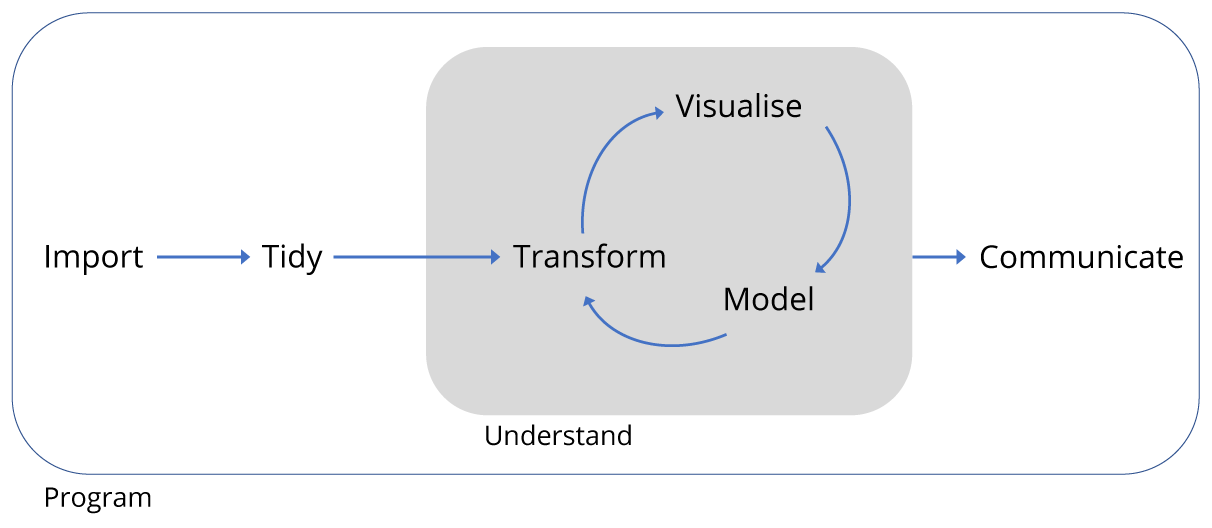
\includegraphics[width=0.8\linewidth]{img/data_project_pipeline} 

}

\caption{Data project workflow.}\label{fig:pipeline}
\end{figure}

As shown in Figure \ref{fig:pipeline} of typical data analysis workflow,
to acheive this aim we need to learn tools that enable us to perform the
fundamental tasks of tasks of importing, tidying and often transforming
the data. Transformation means for example, selecting a subset of the
data to work with, or calculating the mean of a set of observations.
We'll cover that in Chapter \ref{transform}.

But first\ldots{}

\section{What are R and RStudio?}\label{what-are-r-and-rstudio}

\textbf{\emph{``There are only two kinds of languages: the ones people
complain about and the ones nobody uses''}}

\emph{Bjarne Stroustrup}

\textbf{R} is a programming language that follows the philosophy laid
down by it's predecessor S. The philosophy being that users begin in an
interactive environment where they don't consciously think of themselves
as programming. It was created in 1993, and documented in
\citep{ihaka1996}.

Reasons R has become popular include that it is both open source and
cross platform, and that it has broad functionality, from the analysis
of data and creating powerful graphical visualisations and web apps.

Like all languages though it has limitations, for example the syntax is
initially confusing.

Take for example the word \texttt{environment}\ldots{}

\subsection{Environments}\label{environments}

An environment is where we bring our data to work with it. Here we work
in a R envrionment, using the R language as a set of tools.
\textbf{RStudio} is an integrated development environment, or IDE for R
programming. It is regularly updated, and upgrading enables access to
the latest features.

The latest version can be downloaded here:
\url{http://www.rstudio.com/download}

\section{Why learn R, or any language
?}\label{why-learn-r-or-any-language}

We can write R code without saving it, but it's generally more useful to
write and save our code as a script. Working with scripts makes the
steps you used in your analysis clear, and the code you write can be
inspected by someone else who can give you feedback and spot mistakes.

Learning R (or any programming language) and working with scripts forces
you to have deeper understanding of what you are doing, facilitates your
learning and comprehension of the methods you use:

\begin{itemize}
\tightlist
\item
  Writing and publishing code is important for reproducible resarch
\item
  R has many thousands of packages covering many disciplines.
\item
  R can work with many types of data.
\item
  They is a large R community for development and support.
\item
  Using R gives you control over your figures and reports.
\end{itemize}

\section{Finding your way around
RStudio}\label{finding-your-way-around-rstudio}

Let's begin by learning about \href{https://www.rstudio.com/}{RStudio},
the Integrated Development Environment (IDE).

We will use R Studio IDE to write code, navigate the files found on our
computer, inspect the variables we are going to create, and visualize
the plots we will generate. R Studio can also be used for other things
(e.g., version control, developing packages, writing Shiny apps) that we
don't have time to cover during this workshop.

R Studio is divided into ``Panes'', see Figure \ref{fig:rstudio}.

When you first open it, there are three panes,the console where you type
commands, your environment/history (top-right), and your
files/plots/packages/help/viewer (bottom-right).

The enivronment shows all the R objects you have created or are using,
such as data you have imported.

The output pane can be used to view any plots you have created.

Not opened at first start up is the fourth default pane: the script
editor pane, but this will open as soon as we create/edit a R script (or
many other document types). \emph{The script editor is where will be
typing much of the time.}



\begin{figure}

{\centering 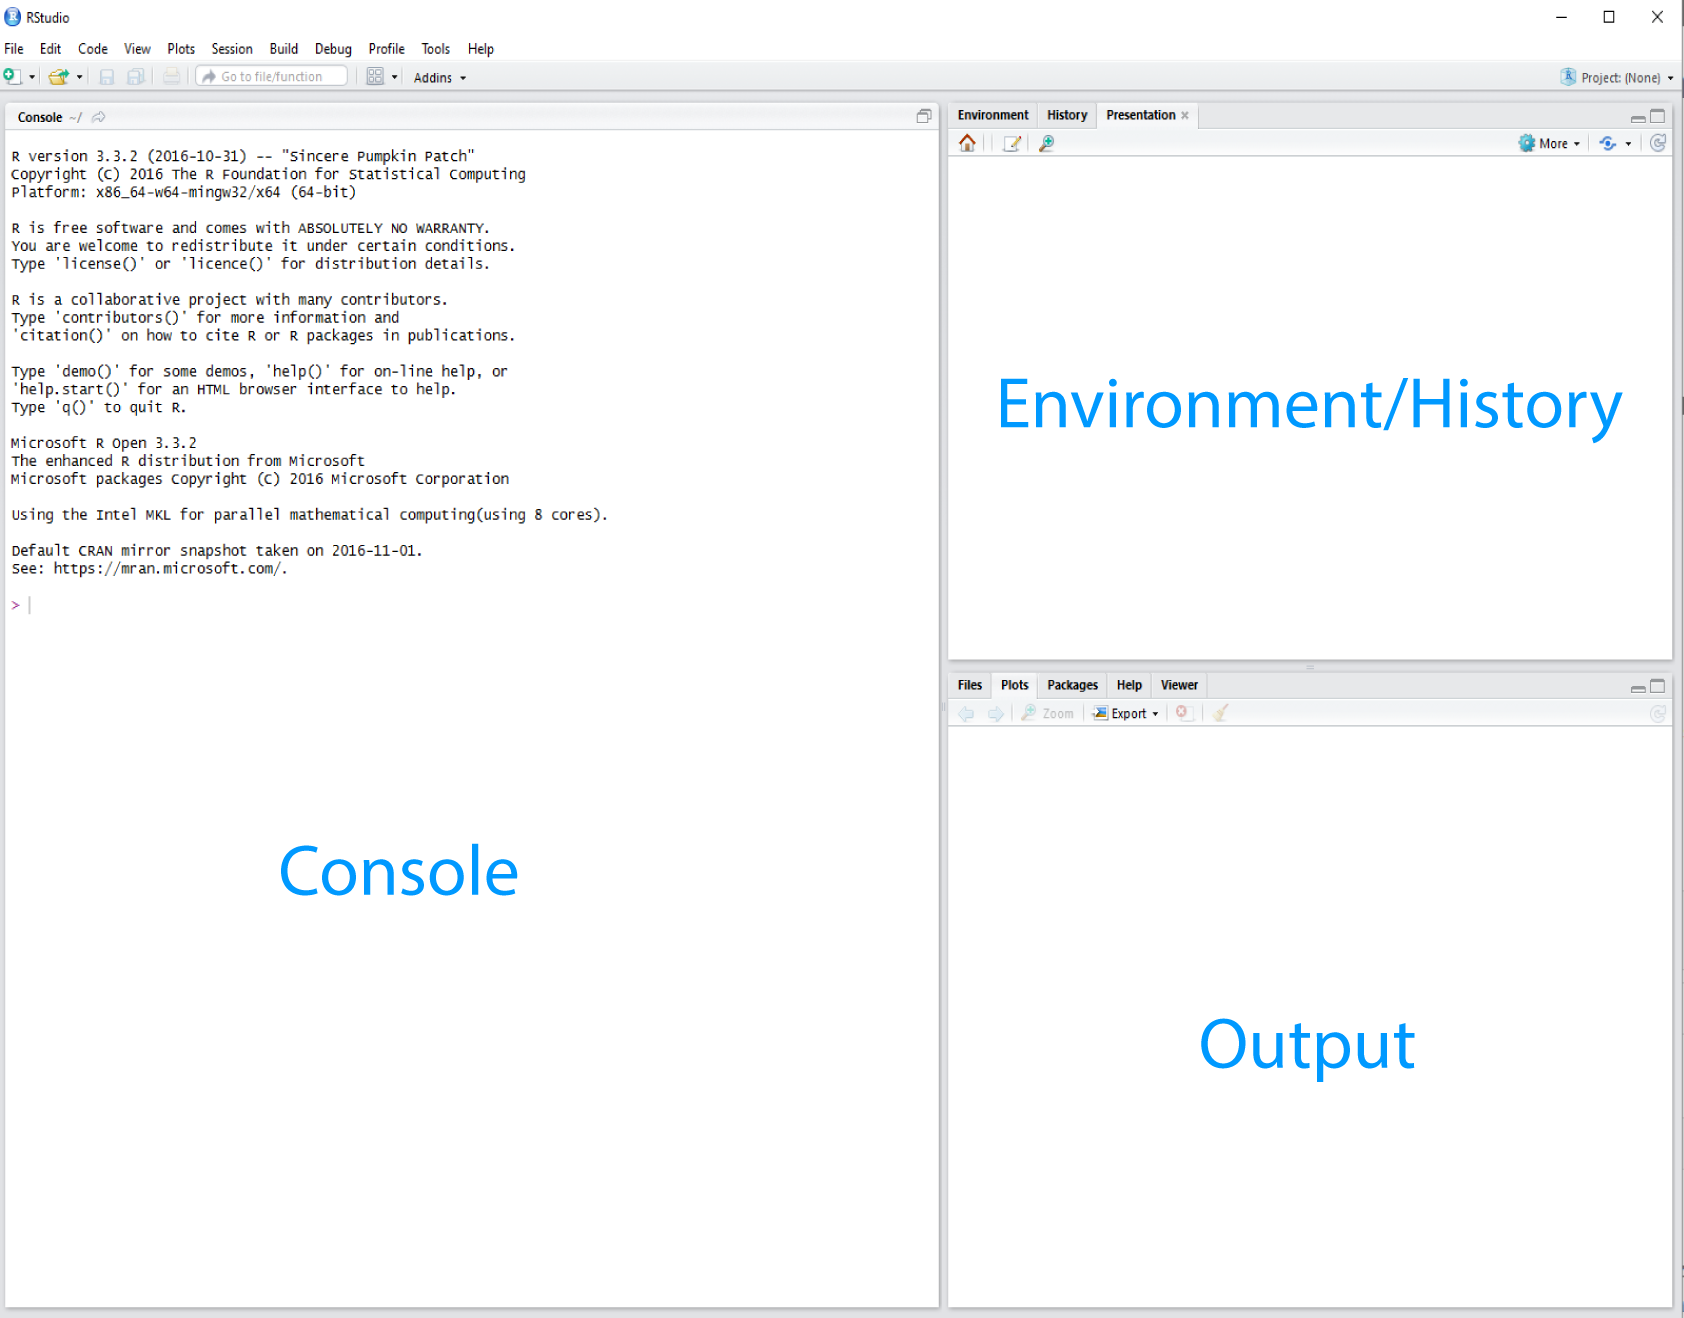
\includegraphics[width=0.8\linewidth]{img/rstudio_ide_image} 

}

\caption{The Rstudio Integrated Development Environment (IDE).}\label{fig:rstudio}
\end{figure}

The placement of these panes and their content can be customized (see
menu, R Studio -\textgreater{} Tools -\textgreater{} Global Options
-\textgreater{} Pane Layout). One of the advantages of using R Studio is
that all the information you need to write code is available ina single
window. Additionally, with many shortcuts, auto-completion, and
highlighting for the major file types you use while developing in R, R
Studio will make typing easier and less error-prone.

Time for a philosphical diversion\ldots{}

\subsection{What is real?}\label{what-is-real}

At the start, we might consider our environment ``real'' - that is to
say the objects we've created/loaded and are using are ``real''. But
it's much better in the long run to consider our scripts as ``real'' -
our scripts are where we write down the code that creates our objects
that we'll be using in our environment.

\textbf{As a script is a document, it is reproducible}

Or to put it another way: we can easily recreate an environment from our
scripts, but not so easily create a script from an enivronment.

To support this notion of thinking in terms of our scripts as real, we
recommend turning off the preservation of workspaces between sessions by
setting the Tools \textgreater{} Global Options menu in R studio as
shown in Figure @\ref(fig:turn-off):



\begin{figure}

{\centering 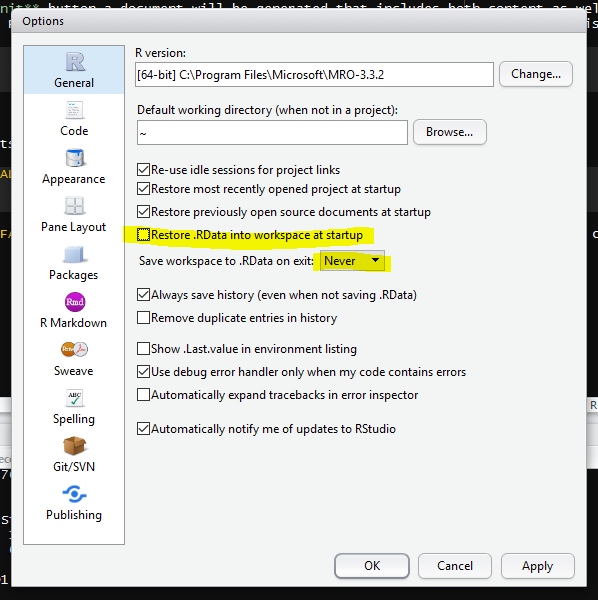
\includegraphics[width=0.8\linewidth]{img/rdata_turn_off} 

}

\caption{Don't save your workspace!}\label{fig:workspace}
\end{figure}

\section{Where am I?}\label{where-am-i}

R studio tells you where you are in terms of directory address like so:

(ref:working-dir)

\begin{figure}

{\centering 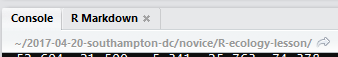
\includegraphics[width=0.8\linewidth]{img/rstudio_working_directory} 

}

\caption{(ref:working-dir)}\label{fig:working-directory}
\end{figure}

If you are unfamiliar with how computers structure folders and files,
then consider a tree with a root from which the trunk extends and
branches divide. In the image above, the \textasciitilde{} symbol
represents a contraction of the path from the root to the `home'
directory (in Windows this is `Documents') and then the forward slashes
are the branches. (Note: Windows uses backslashes, Unix type systems and
R use forwardslashes).

It is good practice to keep a set of related data, analyses, and text
self-contained in a single folder, called the \textbf{working
directory}. All of the scripts within this folder can then use
\emph{relative paths} to files that indicate where inside the project a
file is located (as opposed to absolute paths, which point to where a
file is on a specific computer). Working this way makes it a lot easier
to move your project around on your computer and share it with others
without worrying about whether or not the underlying scripts will still
work.



\begin{figure}

{\centering 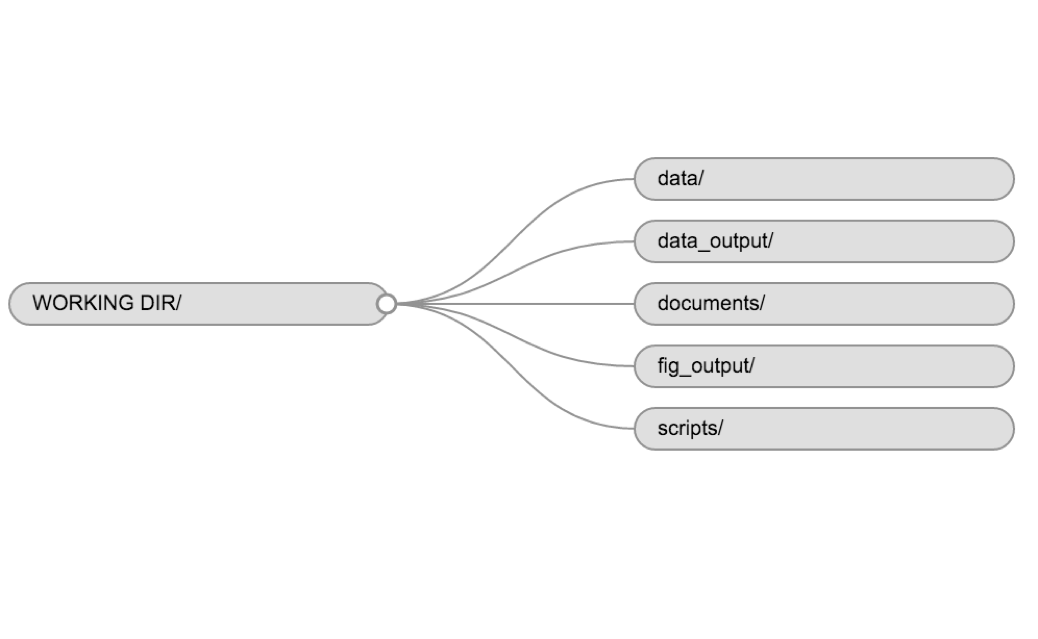
\includegraphics[width=0.8\linewidth]{img/R-ecology-work_dir_structure} 

}

\caption{A typical directory structure}\label{fig:dir-structure}
\end{figure}

\section{R projects}\label{r-projects}

RStudio also has a facility to keep all files associated with a
particular analysis together called a project.

Creating a project creates a working directory for you and also
remembers its location (allowing you to quickly navigate to it) and
optionally preserves custom settings and open files to make it easier to
resume work after a break.

(ref:r-projects)

\begin{figure}

{\centering 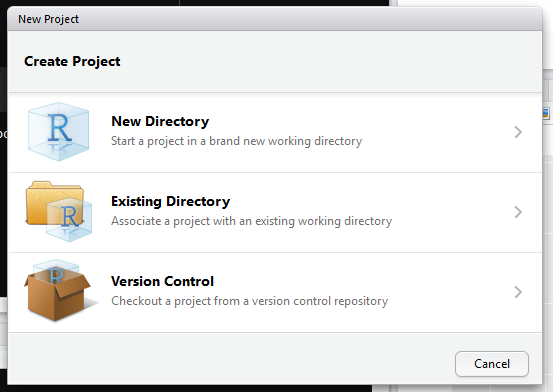
\includegraphics[width=0.8\linewidth]{img/rstudio_create_project} 

}

\caption{(ref:r-projects)}\label{fig:r-projects}
\end{figure}

Below, we will go through the steps for creating an ``R Project'':

\begin{itemize}
\tightlist
\item
  Start R Studio (presentation of R Studio -below- should happen here)
\item
  Under the \texttt{File} menu, click on \texttt{New\ project}, choose
  \texttt{New\ directory}, then \texttt{Empty\ project}
\item
  Enter a name for this new folder (or ``directory'', in computer
  science), and choose a convenient location for it. This will be your
  \textbf{working directory} for the rest of the day (e.g.,
  \texttt{\textasciitilde{}/bspr-workshop})
\item
  Click on ``Create project''
\item
  Under the \texttt{Files} tab on the right of the screen, click on
  \texttt{New\ Folder} and create a folder named \texttt{data} within
  your newly created working directory. (e.g.,
  \texttt{\textasciitilde{}/bspr-workshopdata})
\item
  Create a new R script (File \textgreater{} New File \textgreater{} R
  script) and save it in your working directory (e.g.
  \texttt{bspr-workshop-script.R})
\end{itemize}

\hypertarget{names}{\section{Naming things}\label{names}}

\href{https://ropensci.org/blog/2017/12/08/rprofile-jenny-bryan/}{Jenny
Bryan} has three principles for
\href{http://www2.stat.duke.edu/~rcs46/lectures_2015/01-markdown-git/slides/naming-slides/naming-slides.pdf}{naming
things} that are well worth remembering.

When you names something, a file or an object, ideally it should be:

\begin{enumerate}
\def\labelenumi{\arabic{enumi}.}
\tightlist
\item
  Machine readable (no whitespace, punctuation, upper AND
  lowercase\ldots{})
\item
  Human readable (makes sense in 6 months or 2 years time)
\item
  Plays well with default ordering (numerical or date order)
\end{enumerate}

\section{Seeking help}\label{seeking-help}

If you need help with a specific R function, let's say
\texttt{barplot()}, you can type:

\begin{Shaded}
\begin{Highlighting}[]
\NormalTok{?barplot}
\end{Highlighting}
\end{Shaded}

If you can't find what you are looking for, you can use the
\href{http://www.rdocumentation.org}{rdocumention.org} website that
searches through the help files across all packages available.

A Google or internet search ``R \textless{}task\textgreater{}'' will
often either send you to the appropriate package documentation or a
helpful forum question that someone else already asked, such as
\href{http://stackoverflow.com/questions/tagged/r}{Stack Overflow}.

\subsection{Asking for help}\label{asking-for-help}

As well as knowing
\href{https://www.tidyverse.org/help/\#where-to-ask}{where to ask}, the
key to get help from someone is for them to grasp your problem rapidly.
You should make it as easy as possible to pinpoint where the issue might
be.

Try to use the correct words to describe your problem. For instance, a
package is not the same thing as a library. Most people will understand
what you meant, but others have really strong feelings about the
difference in meaning. The key point is that it can make things
confusing for people trying to help you. Be as precise as possible when
describing your problem.

If possible, try to reduce what doesn't work to a simple
\emph{reproducible example} otherwise known as a \emph{reprex}.

For more information on how to write a reproducible example see
\href{https://www.tidyverse.org/help/\#reprex}{this article}.

\chapter{Getting started in R and the tidyverse}\label{tidyverse}

\section{Tidy data and the tidyverse}\label{tidy-data-and-the-tidyverse}

R is a programming language, and written in R is \emph{``an opinionated
collection of R packages designed for data science''} called
\href{https://www.tidyverse.org/}{tidyverse} \citep{R-tidyverse}.

Tidyverse packages \emph{``share an underlying design philosophy,
grammar, and data structures.''} It's this philiosophy that makes them
relatively easy to learn and use.

The principals of tidy data for tabular data as proposed in the Tidy
Data paper \url{http://www.jstatsoft.org/v59/i10/paper} are:

\begin{enumerate}
\def\labelenumi{\arabic{enumi}.}
\tightlist
\item
  Every variable has its own column.
\item
  Every observation has its own row.
\item
  Each value has its own cell.
\end{enumerate}

If our table was proteomics data then, we might have a set of variables
such as the peptide sequence, mass or length observed for a number of
peptides. Therefore each peptide would have a row with columns for
peptide sequence, mass and length with the value for each variable in
separate cells, as seen in Figure \ref{fig:tidy-prot}.



\begin{figure}

{\centering 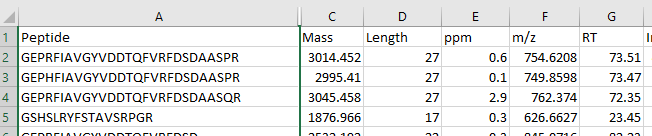
\includegraphics[width=0.8\linewidth]{img/tidy_prot_data} 

}

\caption{An example of tidy proteomics data}\label{fig:tidy-prot}
\end{figure}

We can't do everything in the tidyverse, and everything we can do in the
tidyverse can be done in what is called base R or other packages, but
the motivation behind the tidyverse is to ease the pain of data
manipulation.

With this in mind, the two tasks we are most likely to want to do in
data science are:

\begin{enumerate}
\def\labelenumi{\arabic{enumi}.}
\tightlist
\item
  Visualise our data
\item
  Automate our processes.
\end{enumerate}

Taking our cue from \href{http://r4ds.had.co.nz/}{R4DS} let's try an
example.

\section{Data visualisation}\label{data-visualisation}

Let's begin with visualisation of some data using the \texttt{ggplot2}
package, which implements the \emph{grammer of graphics}, for describing
and building graphs.

The motivation here is twofold: to begin to grasp the grammar of
graphics approach to creating plots, and most importantly to demonstrate
how plotting is often the most useful thing we can do when trying to
understand what is going on.

We'll use the \texttt{mpg} dataset that comes with the tidyverse to
examine the question \emph{do cars with big engines use more fuel than
cars with small engines?}

Try \texttt{?mpg} to learn more about the data.

\begin{enumerate}
\def\labelenumi{\arabic{enumi}.}
\tightlist
\item
  Engine size in litres is in the \texttt{displ} column.
\item
  Fuel efficiency on the highway in miles per gallon is given in the
  \texttt{hwy} column.
\end{enumerate}

To create a plot of engine size \texttt{displ} (x-axis) against fuel
efficiency \texttt{hwy} (y-axis) we do the following:

\begin{enumerate}
\def\labelenumi{\arabic{enumi}.}
\tightlist
\item
  Use the \texttt{ggplot()} function to create an empty graph.
\item
  We give ggplot a first argument of the data (here \texttt{mpg}).
\item
  Then we follow the ggplot function with a \texttt{+} sign to indicate
  we are going to add more coed, followed by a \texttt{geom\_point()}
  function to add a layer of points mapping some aesthetics for the x
  and y axes.
\item
  Mapping is always paired to aesthetics \texttt{aes()}. An aesthetic is
  a visual property of the objects in your plot, such a point size,
  shape or point colour.
\end{enumerate}

Therefore to plot engine size (x-axis) against fuel efficiency (y-axis)
we use the following code:

\begin{Shaded}
\begin{Highlighting}[]
\KeywordTok{ggplot}\NormalTok{(}\DataTypeTok{data =}\NormalTok{ mpg) }\OperatorTok{+}\StringTok{ }
\StringTok{  }\KeywordTok{geom_point}\NormalTok{(}\DataTypeTok{mapping =} \KeywordTok{aes}\NormalTok{(}\DataTypeTok{x =}\NormalTok{ displ, }\DataTypeTok{y =}\NormalTok{ hwy))}
\end{Highlighting}
\end{Shaded}

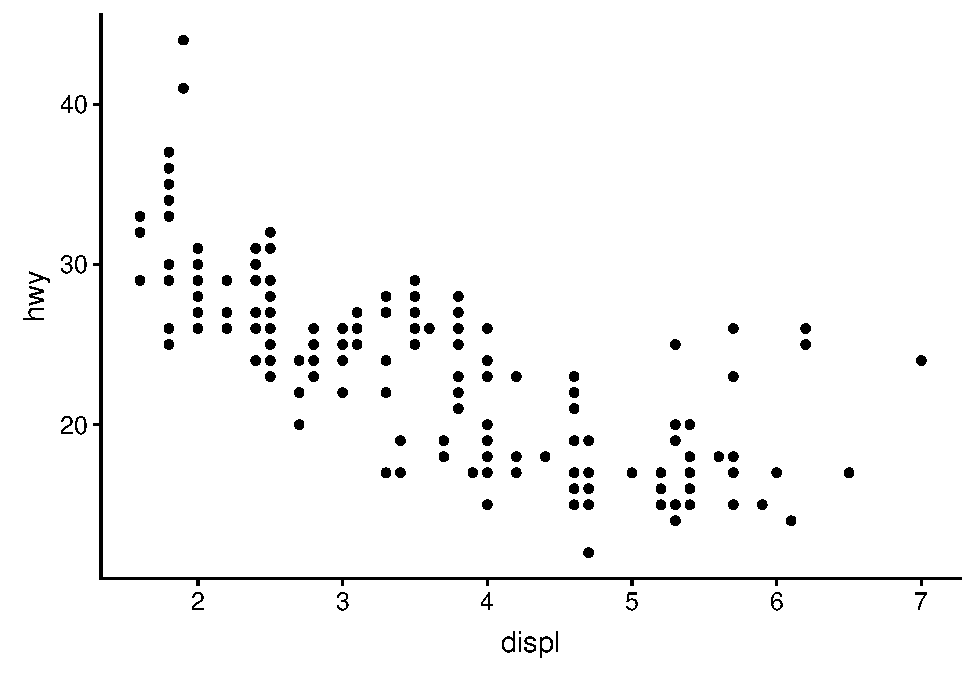
\includegraphics{bspr-workshop-2018_files/figure-latex/mpg-plot-1,mpg_point_plot-1.pdf}

This plot shows a negative relationship between engine size and fuel
efficiency.

Now try extending this code to include to add a \texttt{colour}
aesthetic to the the \texttt{aes()} function, let
\texttt{colour\ =\ class}, \texttt{class} being the veichle type. This
should create a plot with as before but with the points coloured
according to the viechle type to expand our understanding.

\begin{Shaded}
\begin{Highlighting}[]
\KeywordTok{ggplot}\NormalTok{(}\DataTypeTok{data =}\NormalTok{ mpg) }\OperatorTok{+}\StringTok{ }
\StringTok{  }\KeywordTok{geom_point}\NormalTok{(}\DataTypeTok{mapping =} \KeywordTok{aes}\NormalTok{(}\DataTypeTok{x =}\NormalTok{ displ, }\DataTypeTok{y =}\NormalTok{ hwy, }\DataTypeTok{colour =}\NormalTok{ class))}
\end{Highlighting}
\end{Shaded}

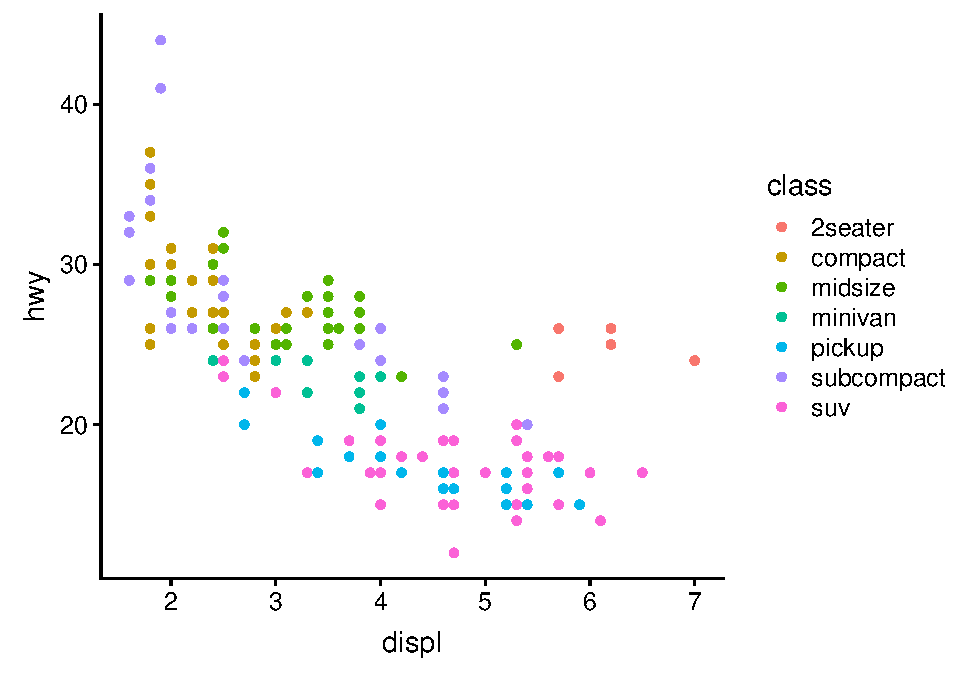
\includegraphics{bspr-workshop-2018_files/figure-latex/mpg-plot-2-1.pdf}

Now we can see that as we might expect, bigger cars such as SUVs tend to
have bigger engines and are also less fuel efficient, but some smaller
cars such as 2-seaters also have big engines and greater fuel
efficiency. Hence we have a more nuanced view with this additional
aesthetic.

Check out the ggplot2 documentation for all the aesthetic possibilities
(and Google for examples): \url{http://ggplot2.tidyverse.org/reference/}

So now we have re-usable code snippet for generating plots in R:

\begin{Shaded}
\begin{Highlighting}[]
\KeywordTok{ggplot}\NormalTok{(}\DataTypeTok{data =} \OperatorTok{<}\NormalTok{DATA}\OperatorTok{>}\NormalTok{) }\OperatorTok{+}\StringTok{ }
\StringTok{  }\ErrorTok{<}\NormalTok{GEOM_FUNCTION}\OperatorTok{>}\NormalTok{(}\DataTypeTok{mapping =} \KeywordTok{aes}\NormalTok{(}\OperatorTok{<}\NormalTok{MAPPINGS}\OperatorTok{>}\NormalTok{))}
\end{Highlighting}
\end{Shaded}

Concretely, in our first example \texttt{\textless{}DATA\textgreater{}}
was \texttt{mpg}, the \texttt{\textless{}GEOM\_FUNCTION\textgreater{}}
was \texttt{geom\_point()} and the arguments we supplies to map our
aesthetics \texttt{\textless{}MAPPINGS\textgreater{}} were
\texttt{x\ =\ displ,\ y\ =\ hwy}.

Hopefully you are beginning to see how a single line of code can do a
lot with tidy data.

\section{Workflow basics}\label{workflow-basics}

Let's run through the basics of working in R to conclude this chapter.

\subsection{Assigning objects}\label{assigning-objects}

Objects are just a way to store data inside the R environment. We create
objects using the assignment operator \texttt{\textless{}-}:

\begin{Shaded}
\begin{Highlighting}[]
\NormalTok{mass_kg <-}\StringTok{ }\DecValTok{55}
\end{Highlighting}
\end{Shaded}

Read this as \emph{``mass\_kg gets value 55''} in your head.

Using \texttt{\textless{}-} can be annoying to type, so use RStudio's
keyboard short cut: Alt + - (the minus sign) to make life easier.

Object name style is a matter of choice, but must start with a letter
and can only contain letters, numbers, \texttt{\_} and \texttt{.}. We
recommend using descriptive names and using \texttt{\_} between words.
Some special symbols cannot be used in variable names, so watch out for
those.

So here we've used the name to indicate its value represents a mass in
kilograms. Look in your environment pane and you'll see the
\texttt{mass\_kg} object containing the (data) value 55.

We can inspect an object by typing it's name:

\begin{Shaded}
\begin{Highlighting}[]
\NormalTok{mass_kg}
\end{Highlighting}
\end{Shaded}

\begin{verbatim}
## [1] 55
\end{verbatim}

What's wrong here?

\begin{Shaded}
\begin{Highlighting}[]
\NormalTok{mass_KG}
\end{Highlighting}
\end{Shaded}

\texttt{Error:\ object\ \textquotesingle{}mass\_KG\textquotesingle{}\ not\ found}

This error illustrates that typos matter, everything must be precise and
\texttt{mass\_KG} is not the same as \texttt{mass\_kg}.
\texttt{mass\_KG} doesn't exist, hence the error.

\subsection{Calling functions}\label{calling-functions}

Functions in R are objects followed by parentheses, such as
\texttt{library()}. Functions have the form:

\texttt{function\_name(arg1\ =\ val,\ arg2\ =\ val2,\ ...)}

Let's use \texttt{seq()} to create a \textbf{seq}uence of numbers, and
at the same time practice tab completion.

Start typing \texttt{se} in the console and you should see a list of
functions appear, add \texttt{q} to shorten the list, then use the up
and down arrow to highlight the function of interest \texttt{seq()} and
hit Tab to select.

RStudio puts the cursor between the parentheses to prompt us to enter
some arguments. Here we'll use 1 as the start and 10 as the end:

\begin{Shaded}
\begin{Highlighting}[]
\KeywordTok{seq}\NormalTok{(}\DecValTok{1}\NormalTok{,}\DecValTok{10}\NormalTok{)}
\end{Highlighting}
\end{Shaded}

\begin{verbatim}
##  [1]  1  2  3  4  5  6  7  8  9 10
\end{verbatim}

If we left off a parentheses to close the function, then when we hit
enter we'll see a \texttt{+} indicating RStudio is expecting further
code. We either add the missing part or press Escape to cancel the code.

Let's call a function and make an assignment at the same time. Here
we'll use the base R function \texttt{seq()} which takes three
arguments: \texttt{from}, \texttt{to} and \texttt{by}.

Read the following code as *``make an object called my\_sequence that
stores a sequence of numbers from 2 to 20 by intervals of 2*.

\begin{Shaded}
\begin{Highlighting}[]
\NormalTok{my_sequence <-}\StringTok{ }\KeywordTok{seq}\NormalTok{(}\DecValTok{2}\NormalTok{,}\DecValTok{20}\NormalTok{,}\DecValTok{2}\NormalTok{)}
\end{Highlighting}
\end{Shaded}

This time nothing was returned to the console, but we now have an object
called \texttt{my\_sequence} in our environment.

Can you remember how to inspect it?

If we want to subset elements of \texttt{my\_sequence} we use square
brackets \texttt{{[}{]}}.

For example element five would be subset by:

\begin{Shaded}
\begin{Highlighting}[]
\NormalTok{my_sequence[}\DecValTok{5}\NormalTok{]}
\end{Highlighting}
\end{Shaded}

\begin{verbatim}
## [1] 10
\end{verbatim}

Here the number five is the index of the vector, not the value of the
fifth element. The value of the fifth element is 10.

And returning multiple elements uses a colon \texttt{:}, like so

\begin{Shaded}
\begin{Highlighting}[]
\NormalTok{my_sequence[}\DecValTok{5}\OperatorTok{:}\DecValTok{8}\NormalTok{]}
\end{Highlighting}
\end{Shaded}

\begin{verbatim}
## [1] 10 12 14 16
\end{verbatim}

\subsection{Atomic vectors}\label{atomic-vectors}

We actually made an atomic vector already when we made
\texttt{my\_sequence}. We made a a one dimensional group of numbers, in
a sequence from two to twenty.

We're not going to be working much with atomic vectors in this workshop,
but to make you aware of how R stores data, atomic vector types are:

\begin{itemize}
\tightlist
\item
  Doubles: regular numbers, +ve or -ve and with or without decimal
  places. AKA numerics.
\item
  Integers: whole numbers, specified with an upper-case L, e.g.
  \texttt{int\ \textless{}-\ 2L}
\item
  Characters: Strings of text
\item
  Logicals: these store \texttt{TRUE}s and \texttt{FALSE}s which are
  useful for comparisons.
\item
  Complex: this would be a vector of numbers with imaginary terms.
\item
  Raw: these vectors store raw bytes of data.
\end{itemize}

Let's make a character vector and check the type:

\begin{Shaded}
\begin{Highlighting}[]
\NormalTok{cards <-}\StringTok{ }\KeywordTok{c}\NormalTok{(}\StringTok{"ace"}\NormalTok{, }\StringTok{"king"}\NormalTok{, }\StringTok{"queen"}\NormalTok{, }\StringTok{"jack"}\NormalTok{, }\StringTok{"ten"}\NormalTok{)}

\NormalTok{cards}
\end{Highlighting}
\end{Shaded}

\begin{verbatim}
## [1] "ace"   "king"  "queen" "jack"  "ten"
\end{verbatim}

\begin{Shaded}
\begin{Highlighting}[]
\KeywordTok{typeof}\NormalTok{(cards)}
\end{Highlighting}
\end{Shaded}

\begin{verbatim}
## [1] "character"
\end{verbatim}

\subsection{Attributes}\label{attributes}

An attribute is a piece of information you can attach to an object, such
as names or dimensions. Attributes such as dimensions are added when we
create an object, but others such as names can be added.

Let's look at the \texttt{mpg} data frame dimensions:

\begin{Shaded}
\begin{Highlighting}[]
\CommentTok{# mpg has 234 rows (observations) and 11 columns (variables)}
\KeywordTok{dim}\NormalTok{(mpg)}
\end{Highlighting}
\end{Shaded}

\begin{verbatim}
## [1] 234  11
\end{verbatim}

\subsection{Factors}\label{factors}

Factors are Rs way of storing categorical information such as eye colour
or car type. A factor is something that can only have certain values,
and can be ordered (such as \texttt{low},\texttt{medium},\texttt{high})
or unordered such as types of fruit.

Factors are useful as they code string variables such as ``red'' or
``blue'' to integer values e.g.~1 and 2, which can be used in
statistical models and when plotting, but they are confusing as they
look like strings.

\textbf{Factors look like strings, but behave like integers.}

Historically R converts strings to factors when we load and create data,
but it's often not what we want as a default. Fortunately, in the
tidyverse strings are not treated as factors by default.

\subsection{Lists}\label{lists}

Lists also group data into one dimensional sets of data. The difference
being that list group objects instead of individual values, such as
several atomic vectors.

For example, let's make a list containing a vector of numbers and a
character vector

\begin{Shaded}
\begin{Highlighting}[]
\NormalTok{list_}\DecValTok{1}\NormalTok{ <-}\StringTok{ }\KeywordTok{list}\NormalTok{(}\DecValTok{1}\OperatorTok{:}\DecValTok{110}\NormalTok{,}\StringTok{"R"}\NormalTok{)}

\NormalTok{list_}\DecValTok{1}
\end{Highlighting}
\end{Shaded}

\begin{verbatim}
## [[1]]
##   [1]   1   2   3   4   5   6   7   8   9  10  11  12  13  14  15  16  17
##  [18]  18  19  20  21  22  23  24  25  26  27  28  29  30  31  32  33  34
##  [35]  35  36  37  38  39  40  41  42  43  44  45  46  47  48  49  50  51
##  [52]  52  53  54  55  56  57  58  59  60  61  62  63  64  65  66  67  68
##  [69]  69  70  71  72  73  74  75  76  77  78  79  80  81  82  83  84  85
##  [86]  86  87  88  89  90  91  92  93  94  95  96  97  98  99 100 101 102
## [103] 103 104 105 106 107 108 109 110
## 
## [[2]]
## [1] "R"
\end{verbatim}

Note the double brackets to indicate the list elements, i.e.~element one
is the vector of numbers and element two is a vector of a single
character.

We won't be working with lists in this workshop, but they are a flexible
way to store data of different types in R.

Accessing list elements uses double square brackets syntax, for example
\texttt{list\_1{[}{[}1{]}{]}} would return the first vector in our list.

And to access the first element in the first vector would combine double
and single square brackets like so:
\texttt{list\_1{[}{[}1{]}{]}{[}1{]}}.

Don't worry if you find this confusing, everyone does when they first
start with R.

\subsection{Matrices and arrays}\label{matrices-and-arrays}

Matrices store values in a two dimensional array, whilst arrays can have
n dimensions. We won't be using these either, but they are also valid R
objects.

\subsection{Data frames}\label{data-frames}

Data frames are two dimensional versions of lists, and this is form of
storing data we are going to be using. In a data frame each atomic
vector type becomes a column, and a data frame is formed by columns of
vectors of the same length. Each column element must be of the same
type, but the column types can vary.

Figure \ref{fig:df} shows an example data frame we'll refer to as saved
as the object \texttt{df} consisting of three rows and three columns.
Each column is a different atomic data type of the same length.



\begin{figure}

{\centering 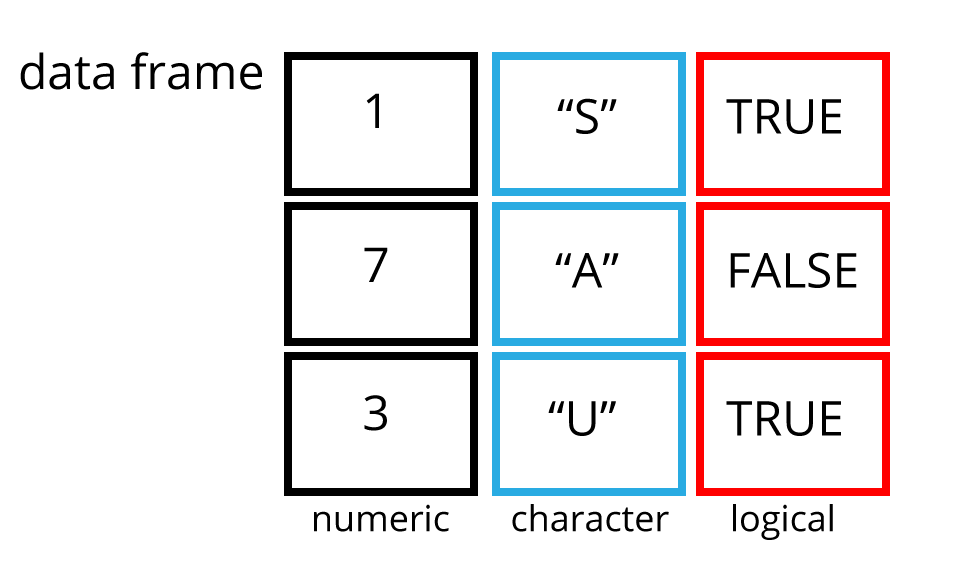
\includegraphics[width=0.8\linewidth]{img/data_frame} 

}

\caption{An example data frame \texttt{df}.}\label{fig:df}
\end{figure}

Packages in the tidyverse create a modified form of data frame called a
tibble. You can read about tibbles
\href{http://r4ds.had.co.nz/tibbles.html}{here}. One advantage of
tibbles is that they don't default to treating strings as factors. We
deal with modifying data frames when we work with our example data set.

Sub-setting data frames can also be done with square bracket syntax, but
as we have both rows and columns, we need to provide index values for
both row and column.

For example \texttt{df{[}1,2{]}} means \textbf{return the value of
\texttt{df} row 1, column 2}. This corresponds with the value
\texttt{A}.

We can also use the colon operator to choose several rows or columns,
and by leaving the row or column blank we return all rows or all
columns.

\begin{Shaded}
\begin{Highlighting}[]
\CommentTok{# Subset rows 1 and 2 of column 1}
\NormalTok{df[}\DecValTok{1}\OperatorTok{:}\DecValTok{2}\NormalTok{,}\DecValTok{1}\NormalTok{]}

\CommentTok{# Subset all rows of column 3}
\NormalTok{df[,}\DecValTok{3}\NormalTok{]}
\end{Highlighting}
\end{Shaded}

Again don't worry too much about this for now, we won't be doing to much
of this in this lesson, but it's important to be aware of the basic
syntax.

\section{Learning more R}\label{learning-more-r}

There are many places to start, but swirl can teach you interactively,
and at your own pace in RStudio.

Just follow the instructions via this link:
\url{http://swirlstats.com/students.html}

\emph{Hands-On Programming with R} by Garrett Grolemund is another great
resource for learning R.

Plus all the \href{https://www.tidyverse.org/learn/}{tidyverse links}.

\chapter{Creating scripts and importing data}\label{import}

Our analysis is of an example data set of observations for 7702 proteins
from cells in three control experiments and three treatment experiments.
The observations are signal intensity measurements from the mass
spectrometer. These intensities relate to the amount of protein in each
experiment and under each condition.

We consider raw data as the data as we receive it. This doesn't mean it
hasn't be processed in some way, it just means it hasn't been processed
by us. Generally speaking we don't change the raw data file, what we do
is import it and create an object in R which we then transform.

So let's understand how to import some data.

\section{Some definitions}\label{some-definitions}

\begin{itemize}
\tightlist
\item
  Importing means getting data into our R environment by turning into
  into a R object that we can then manipulate. The raw data file remains
  unchanged.
\item
  Inspecting means looking at the dataset to understand what it
  contains.
\item
  Tidying refers to getting data into a consistent format that makes it
  easy to use in later steps.
\end{itemize}

A note here is that we are focusing on rectangular data, the sort that
comes in rows and columns such as in a spreadsheet. Lots of our data
types exist, such as images, which are beyond the scope of this lesson,
but can also be handled by R.

\section{Using scripts}\label{using-scripts}

Using the console is useful, but as we build up a workflow, that is to
say, wring code to:

\begin{itemize}
\tightlist
\item
  load packages
\item
  load data
\item
  explore the data
\item
  and output some results
\end{itemize}

Then it's much more useful to contain this in a script: a document of
our code.

Why? When we write and save our code in scripts, we can re-use it, share
it or edit it. But \textbf{most importantly a script is a record}.

Cmd/Ctrl + Shift + N will open a new script file up and you should see
something like Figure \ref{fig:script-pane} with the script editor pane
open:



\begin{figure}

{\centering 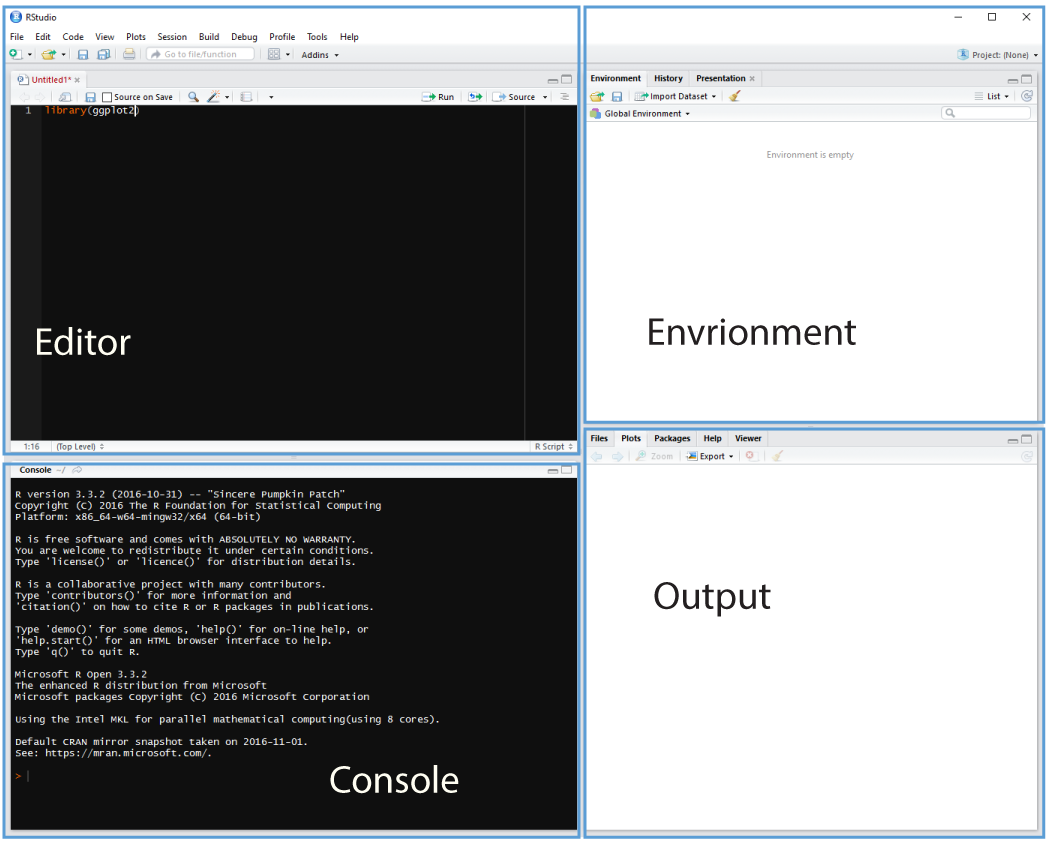
\includegraphics[width=0.8\linewidth]{img/rstudio_screenshot_four_panes} 

}

\caption{Rstudio with the script editor pane open.}\label{fig:script-pane}
\end{figure}

\section{Running code}\label{running-code}

We can run a highlighted portion of code in your script if you click the
Run button at the top of the scripts pane as shown in Figure
\ref{fig:run-script}.

(ref:run-script)

\begin{figure}

{\centering 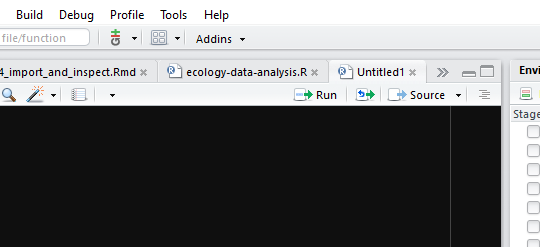
\includegraphics[width=0.8\linewidth]{img/run_script} 

}

\caption{(ref:run-script)}\label{fig:run-script}
\end{figure}

You can run the entire script by clicking the Source button.

Or we can run chunks of code if we split our script into sections, see
below.

\section{Creating a R script}\label{creating-a-r-script}

We first need to create a script that will form the basis of our
analysis.

Go to the file menu and select New Files \textgreater{} R script. This
should open the script editor pane.

Now let's save the script, by going to File \textgreater{} Save and we
should find ourselves prompted to save the script in our Project
Directory.

Following the advice about \protect\hyperlink{names}{naming things} we
can create a new R script called \texttt{01-bspr-workshop-july-2018}.

This name is machine readable (no spaces or special characters), human
readable, and works well with default ordering by beginning with
\texttt{01}.

\section{Setting up our environment}\label{setting-up-our-environment}

At the head of our script it's common to put a title, the name of the
author and the date, and any other useful information. This is created
as comments using the \texttt{\#} at the start of each line.

It's then usual to follow this by code to load the packages we need into
our our R environment using the \texttt{library()} function and
providing the name of the package we wish to load. Packages are
collections of R functions.

Often we break the code up into regions by adding dashes (or equals
symbols) to the comment line. This enables us to run chunks of the
script separately from running the whole script when using our code.

Here is a typical head for a script:

\begin{Shaded}
\begin{Highlighting}[]
\CommentTok{# My workshop script}
\CommentTok{# 7th July 2018}
\CommentTok{# Alistair Bailey}

\CommentTok{# Load packages ----------------------------------------------------------------}
\KeywordTok{library}\NormalTok{(tidyverse)}
\KeywordTok{library}\NormalTok{(gplots)}
\KeywordTok{library}\NormalTok{(pheatmap)}
\end{Highlighting}
\end{Shaded}

\subsection{Bioconductor}\label{bioconductor}

As an aside there are many proteomics specific R packages, these are
generally found through
\href{https://www.bioconductor.org/}{Bioconductor} which is a project
that was initiated in 2001 to create tools for the analysis of
high-throughput genomic data, but also includes other 'omics data tools
\citep[\citet{huber2015}]{gentleman2004}.

Exploring Bioconductor is beyond our scope here, but well worth
exploring for manipulation and analysis of raw data formats such as
mzxml files.

\section{Importing data}\label{importing-data}

Assuming our data is in a flat format, we can import it into our
environment using the tidyverse \texttt{readr} package. A flat format is
a file that contains only text such as \texttt{csv} or tab separated
data without meta-data (extra information), such as the colour of cells
in an excel file.

If we our data was an excel file, we can use the tidyverse
\texttt{readxl} package to import the data.

For the purposes of this workshop we have a \texttt{csv} (comma
separated variable) file.

If you haven't done so already Click here to download the example data
and save it to our project directory. Check the \texttt{Files} pane to
see it's there.

We then import data and assign it to an object we'll call \texttt{data}
like so:

\begin{Shaded}
\begin{Highlighting}[]
\CommentTok{# Import example data ----------------------------------------------------------}
\CommentTok{# Import the example data with read_csv from the readr package}
\NormalTok{dat <-}\StringTok{ }\NormalTok{readr}\OperatorTok{::}\KeywordTok{read_csv}\NormalTok{(}\StringTok{"data/070718-proteomics-example-data.csv"}\NormalTok{)}
\end{Highlighting}
\end{Shaded}

\begin{verbatim}
## Parsed with column specification:
## cols(
##   protein_accession = col_character(),
##   protein_description = col_character(),
##   control_1 = col_double(),
##   control_2 = col_double(),
##   control_3 = col_double(),
##   treatment_1 = col_double(),
##   treatment_2 = col_double(),
##   treatment_3 = col_double()
## )
\end{verbatim}

\section{Exploring the data}\label{exploring-the-data}

The first thing to do with any data set is to actually look at it. Here
are three ways to have look in the \texttt{Console}:

\begin{Shaded}
\begin{Highlighting}[]
\CommentTok{# call object}
\NormalTok{dat}
\end{Highlighting}
\end{Shaded}

\begin{verbatim}
## # A tibble: 7,702 x 8
##    protein_accession protein_description     control_1 control_2 control_3
##    <chr>             <chr>                       <dbl>     <dbl>     <dbl>
##  1 VATA_HUMAN_P38606 V-type proton ATPase c~     0.811     0.858     1.04 
##  2 RL35A_HUMAN_P180~ 60S ribosomal protein ~     0.367     0.385     0.409
##  3 MYH10_HUMAN_P355~ Myosin-10 OS=Homo sapi~     2.98      4.62      2.87 
##  4 RHOG_HUMAN_P84095 Rho-related GTP-bindin~     0.142     0.224     0.128
##  5 PSA1_HUMAN_P25786 Proteasome subunit alp~     1.07      0.945     0.803
##  6 PRDX5_HUMAN_P300~ Peroxiredoxin-5_ mitoc~     0.566     0.540     0.488
##  7 ACLY_HUMAN_P53396 ATP-citrate synthase O~     5.00      4.22      5.03 
##  8 VDAC2_HUMAN_P458~ Voltage-dependent anio~     1.35      1.33      1.14 
##  9 LRC47_HUMAN_Q8N1~ Leucine-rich repeat-co~     0.927     0.770     1.17 
## 10 CH60_HUMAN_P10809 60 kDa heat shock prot~     9.45      8.41     10.4  
## # ... with 7,692 more rows, and 3 more variables: treatment_1 <dbl>,
## #   treatment_2 <dbl>, treatment_3 <dbl>
\end{verbatim}

\begin{Shaded}
\begin{Highlighting}[]
\CommentTok{# tidyverse glimpse function}
\KeywordTok{glimpse}\NormalTok{(dat)}
\end{Highlighting}
\end{Shaded}

\begin{verbatim}
## Observations: 7,702
## Variables: 8
## $ protein_accession   <chr> "VATA_HUMAN_P38606", "RL35A_HUMAN_P18077",...
## $ protein_description <chr> "V-type proton ATPase catalytic subunit A ...
## $ control_1           <dbl> 0.8114, 0.3672, 2.9815, 0.1424, 1.0748, 0....
## $ control_2           <dbl> 0.8575, 0.3853, 4.6176, 0.2238, 0.9451, 0....
## $ control_3           <dbl> 1.0381, 0.4091, 2.8709, 0.1281, 0.8032, 0....
## $ treatment_1         <dbl> 0.6448, 0.4109, 7.1670, 0.1643, 0.7884, 0....
## $ treatment_2         <dbl> 0.7190, 0.4634, 2.0052, 0.2466, 0.8798, 1....
## $ treatment_3         <dbl> 0.4805, 0.3561, 0.8995, 0.1268, 0.7631, 0....
\end{verbatim}

\begin{Shaded}
\begin{Highlighting}[]
\CommentTok{# head function}
\KeywordTok{head}\NormalTok{(dat)}
\end{Highlighting}
\end{Shaded}

\begin{verbatim}
## # A tibble: 6 x 8
##   protein_accession protein_description      control_1 control_2 control_3
##   <chr>             <chr>                        <dbl>     <dbl>     <dbl>
## 1 VATA_HUMAN_P38606 V-type proton ATPase ca~     0.811     0.858     1.04 
## 2 RL35A_HUMAN_P180~ 60S ribosomal protein L~     0.367     0.385     0.409
## 3 MYH10_HUMAN_P355~ Myosin-10 OS=Homo sapie~     2.98      4.62      2.87 
## 4 RHOG_HUMAN_P84095 Rho-related GTP-binding~     0.142     0.224     0.128
## 5 PSA1_HUMAN_P25786 Proteasome subunit alph~     1.07      0.945     0.803
## 6 PRDX5_HUMAN_P300~ Peroxiredoxin-5_ mitoch~     0.566     0.540     0.488
## # ... with 3 more variables: treatment_1 <dbl>, treatment_2 <dbl>,
## #   treatment_3 <dbl>
\end{verbatim}

\begin{Shaded}
\begin{Highlighting}[]
\CommentTok{# str function}
\KeywordTok{str}\NormalTok{(dat)}
\end{Highlighting}
\end{Shaded}

\begin{verbatim}
## Classes 'tbl_df', 'tbl' and 'data.frame':    7702 obs. of  8 variables:
##  $ protein_accession  : chr  "VATA_HUMAN_P38606" "RL35A_HUMAN_P18077" "MYH10_HUMAN_P35580" "RHOG_HUMAN_P84095" ...
##  $ protein_description: chr  "V-type proton ATPase catalytic subunit A OS=Homo sapiens GN=ATP6V1A PE=1 SV=2" "60S ribosomal protein L35a OS=Homo sapiens GN=RPL35A PE=1 SV=2" "Myosin-10 OS=Homo sapiens GN=MYH10 PE=1 SV=3" "Rho-related GTP-binding protein RhoG OS=Homo sapiens GN=RHOG PE=1 SV=1" ...
##  $ control_1          : num  0.811 0.367 2.982 0.142 1.075 ...
##  $ control_2          : num  0.858 0.385 4.618 0.224 0.945 ...
##  $ control_3          : num  1.038 0.409 2.871 0.128 0.803 ...
##  $ treatment_1        : num  0.645 0.411 7.167 0.164 0.788 ...
##  $ treatment_2        : num  0.719 0.463 2.005 0.247 0.88 ...
##  $ treatment_3        : num  0.48 0.356 0.899 0.127 0.763 ...
##  - attr(*, "spec")=List of 2
##   ..$ cols   :List of 8
##   .. ..$ protein_accession  : list()
##   .. .. ..- attr(*, "class")= chr  "collector_character" "collector"
##   .. ..$ protein_description: list()
##   .. .. ..- attr(*, "class")= chr  "collector_character" "collector"
##   .. ..$ control_1          : list()
##   .. .. ..- attr(*, "class")= chr  "collector_double" "collector"
##   .. ..$ control_2          : list()
##   .. .. ..- attr(*, "class")= chr  "collector_double" "collector"
##   .. ..$ control_3          : list()
##   .. .. ..- attr(*, "class")= chr  "collector_double" "collector"
##   .. ..$ treatment_1        : list()
##   .. .. ..- attr(*, "class")= chr  "collector_double" "collector"
##   .. ..$ treatment_2        : list()
##   .. .. ..- attr(*, "class")= chr  "collector_double" "collector"
##   .. ..$ treatment_3        : list()
##   .. .. ..- attr(*, "class")= chr  "collector_double" "collector"
##   ..$ default: list()
##   .. ..- attr(*, "class")= chr  "collector_guess" "collector"
##   ..- attr(*, "class")= chr "col_spec"
\end{verbatim}

To see the data in a \emph{spreadsheet} fashion use \texttt{View(dat)},
note the capital V and a new tab will open. This can also be launched
from the \texttt{Environment} tab by clicking on \texttt{dat}.

Although this provides us with some useful information, such as the
number of observations and variables, to understand more plotting the
data will be helpful as we'll see in Section {[}\#normalisation{]}.

\chapter{Transformation and visualisation}\label{transform}

Having imported our data set of observations for 7702 proteins from
cells in three control experiments and three treatment experiments.
Remember, the observations are signal intensity measurements from the
mass spectrometer, and these intensities relate to the amount of protein
in each experiment and under each condition.

Next we will transform the data to examine the effect of the treatment
on the cellular proteome and visualise the output using a volcano plot
and a heatmap.

\section{Fold change and log-fold
change}\label{fold-change-and-log-fold-change}

Fold changes are ratios, the ratio of say protein expression before and
after treatment, where a value larger than 1 for a protein implies that
protein expression was greater after the treatment.

In life sciences, fold change is often reported as log-fold change. Why
is that? There are at least two reasons which can be shown by plotting.

One is that ratios are not symmetrical around 1, so it's difficult to
observe both changes in the forwards and backwards direcion
i.e.~proteins where expression went up and proteins where expression
went down due to treatment. When we transform ratios on a log scale, the
scale becomes symmetric around 0 and thus we can now observe the
distribution of ratios in terms of positive, negative or no change.




\begin{figure}
\centering
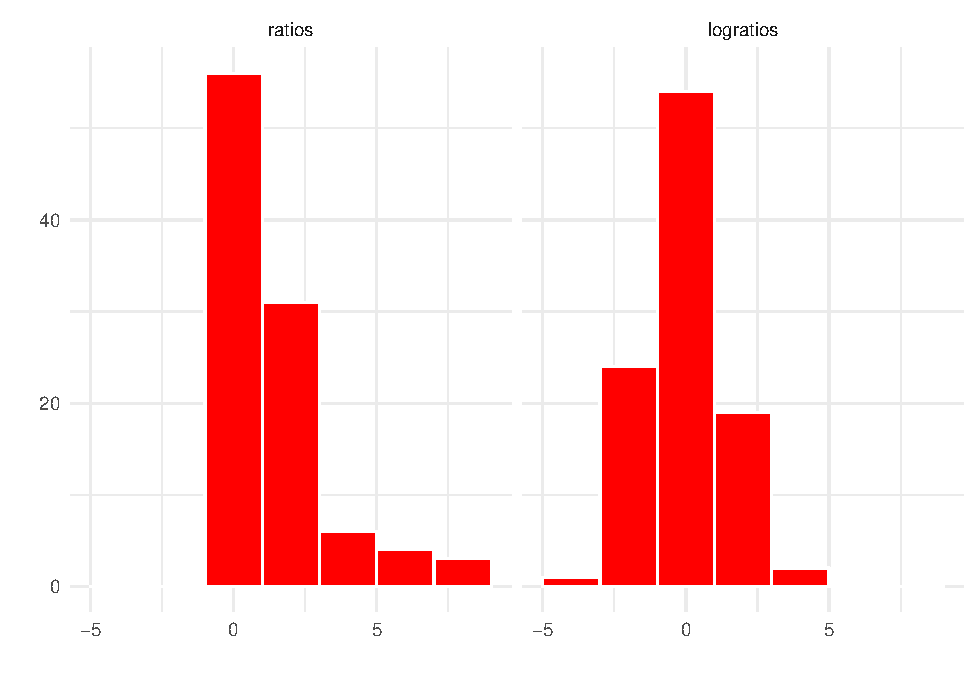
\includegraphics{bspr-workshop-2018_files/figure-latex/fold-change-1-1.pdf}
\caption{\label{fig:fold-change-1}Ratios are not symmetric around one, logratios are
symmetric around zero.}
\end{figure}

A second reason is that transforming values onto a log scale changes
where the numbers actually occur when plotted on that scale. If we
consider the log scale to represent magnitudes, then we can more easily
see changes of small and large magnitudes when we plot the data.

For example, a fold change of 32 times can be either a ratio 1/32 or
32/1.

As shown in Figure \ref{fig:fold-change-2}, 1/32 is much closer to 1
than 32/1, but transformed to a log scale we see that in terms of
magnitude of difference it is the same as 32/1.



\begin{figure}
\centering
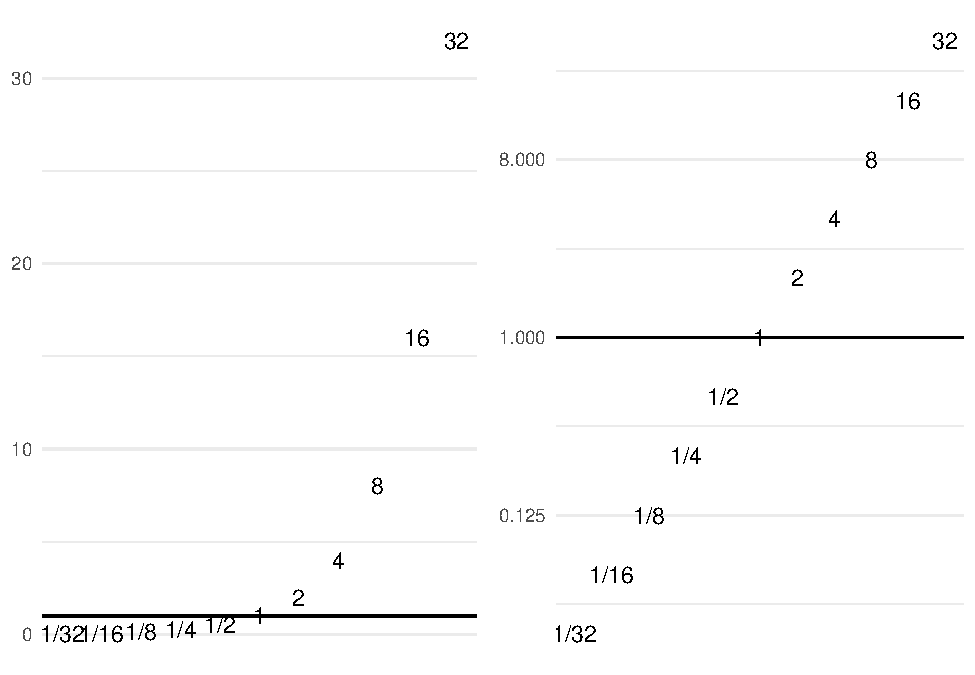
\includegraphics{bspr-workshop-2018_files/figure-latex/fold-change-2-1.pdf}
\caption{\label{fig:fold-change-2}Transformation of scales using log transformation.}
\end{figure}

\section{Dealing with missing values}\label{missing-values}

Unless we're really lucky, it's unlikely that we'll get observations for
the same numbers of proteins in all replicated experiments. This means
there will be missing values for some proteins when looking at all the
experiments together. This then raises the question of what to do about
the missing values? We have two choices:

\begin{enumerate}
\def\labelenumi{\arabic{enumi}.}
\tightlist
\item
  Only analyse the proteins that we have observations for in all
  experiments.
\item
  Impute values for the missing values from the existing observations.
\end{enumerate}

There are pros and cons to either approach. Here for simplicity we'll
use only the proteins for which we have observations in all assays.

We can drop the proteins with missing values by piping our data set to
the \texttt{drop\_na()} function from the \texttt{tidyr} package like
so. We assign this to a new object called \texttt{dat\_tidy}.

\begin{Shaded}
\begin{Highlighting}[]
\CommentTok{# Remove the missing values}
\NormalTok{dat_tidy <-}\StringTok{ }\NormalTok{dat }\OperatorTok\StringTok{ }\KeywordTok{drop_na}\NormalTok{()}

\CommentTok{# Nunber of proteins in original data}
\NormalTok{dat }\OperatorTok\StringTok{ }\KeywordTok{summarise}\NormalTok{(}\DataTypeTok{Number_of_proteins =} \KeywordTok{n}\NormalTok{())}
\end{Highlighting}
\end{Shaded}

\begin{verbatim}
## # A tibble: 1 x 1
##   Number_of_proteins
##                <int>
## 1               7702
\end{verbatim}

\begin{Shaded}
\begin{Highlighting}[]
\CommentTok{# Nunber of proteins without missing values}
\NormalTok{dat_tidy }\OperatorTok\StringTok{ }\KeywordTok{summarise}\NormalTok{(}\DataTypeTok{Number_of_proteins =} \KeywordTok{n}\NormalTok{())}
\end{Highlighting}
\end{Shaded}

\begin{verbatim}
## # A tibble: 1 x 1
##   Number_of_proteins
##                <int>
## 1               1145
\end{verbatim}

This shrinks the dataset from 7,702 proteins to 1,184 proteins, so we
can see why imputing the missing values might be more atrractive.

One approach you might like to try is to impute the data by replacing
the missing values with the mean observation for each protein.

\section{Data normalization}\label{normalisation}

To perform statistical inference, for example whether treatment
increases or decreases protein abundance, we need to account for the
variation that occurs from run to run on our spectrometers and each give
rise to a different distribution. This is as opposed to variation
arising from treatment versus control which we are interested in
understanding. Hence normalization seeks to reduce the run-to-run
sources of variation.

A method of normalization introduced for DNA microarray analysis is
quantile normalization \citep{bolstad2003}.

If we consider our proteomics data as a distribution of values, one
value for the concentration of each protein in our experiment that
together form a distribution. Figure \ref{fig:data-dist} shows the
distribution of protein concentrations observed for the three control
and three treatment assays. As we can see the distributions are
different for each assay.



\begin{figure}

{\centering 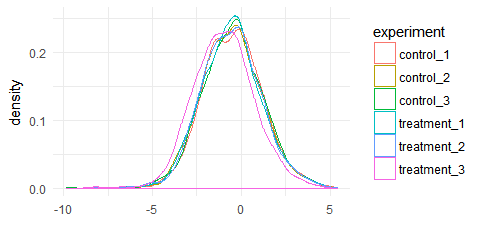
\includegraphics[width=0.8\linewidth]{bspr-workshop-2018_files/figure-latex/data-dist-1} 

}

\caption{Protein data for six assays plotted as a distributions.}\label{fig:data-dist}
\end{figure}

A quantile represents a region of distribution, for example the 0.95
quantile is the value such that 95\% of the data lies below it. To
normalize two or more distributions with each other without recourse to
a reference distribution we:

\begin{enumerate}
\def\labelenumi{(\roman{enumi})}
\tightlist
\item
  Rank the value in each experiment (represented in the columns) from
  lowest to highest. In other words identify the quantiles.
\item
  Sort each experiment (the columns) from lowest to highest value.
\item
  Calculate the mean across the rows for the sorted values.
\item
  Then substitute these mean values back according to rank for each
  experiment to restore the original order.
\end{enumerate}

This results in the highest ranking observation in each experiment
becoming the mean of the highest observations across all experiments,
the second ranking observation in each experiment becoming the mean of
the second highest observations across all experiments.

\href{https://davetang.org/muse/2014/07/07/quantile-normalisation-in-r/}{Dave
Tang's Blog:Quantile Normalisation in R} has more details on this
approach.





\begin{figure}

{\centering 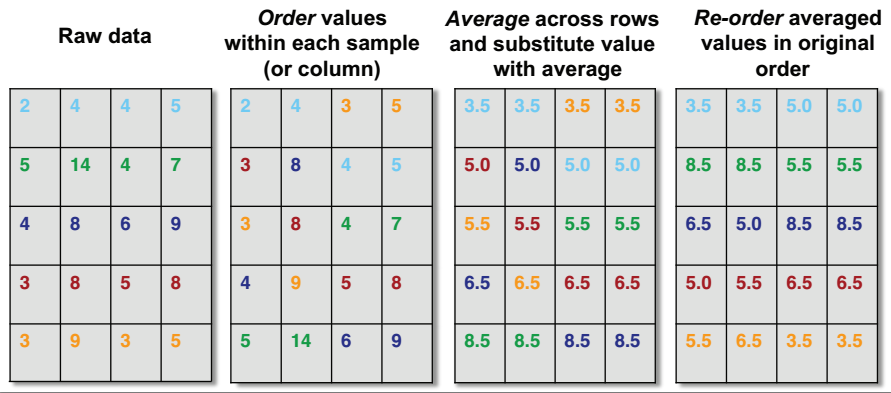
\includegraphics[width=0.8\linewidth]{img/quant_norm} 

}

\caption{Quantile Normalisation from
\href{https://twitter.com/rafalab/status/545586012219772928?ref_src=twsrc\%5Etfw}{Rafael
Irizarry's tweet}.}\label{fig:quant-norm}
\end{figure}

These result of quantile normalization is that our distributions become
statisitcally identitical, which we can see by plotting the densities of
the normalized data. As shown in Figure \ref{fig:compare-normalisation}
the distributions all overlay.

\begin{Shaded}
\begin{Highlighting}[]
\CommentTok{# Quantile normalisation : the aim is to give different distributions the}
\CommentTok{# same statistical properties}
\NormalTok{quantile_normalisation <-}\StringTok{ }\ControlFlowTok{function}\NormalTok{(df)\{}
\NormalTok{  df_rank <-}\StringTok{ }\KeywordTok{apply}\NormalTok{(df,}\DecValTok{2}\NormalTok{,rank,}\DataTypeTok{ties.method=}\StringTok{"average"}\NormalTok{)}
\NormalTok{  df_sorted <-}\StringTok{ }\KeywordTok{data.frame}\NormalTok{(}\KeywordTok{apply}\NormalTok{(df, }\DecValTok{2}\NormalTok{, sort))}
\NormalTok{  df_mean <-}\StringTok{ }\KeywordTok{apply}\NormalTok{(df_sorted, }\DecValTok{1}\NormalTok{, mean)}
   
\NormalTok{  index_to_mean <-}\StringTok{ }\ControlFlowTok{function}\NormalTok{(my_index, my_mean)\{}
    \KeywordTok{return}\NormalTok{(my_mean[my_index])}
\NormalTok{  \}}
   
\NormalTok{  df_final <-}\StringTok{ }\KeywordTok{apply}\NormalTok{(df_rank, }\DecValTok{2}\NormalTok{, index_to_mean, }\DataTypeTok{my_mean=}\NormalTok{df_mean) }\OperatorTok\StringTok{ }
\StringTok{    }\KeywordTok{as.tibble}\NormalTok{()}
  
  \KeywordTok{return}\NormalTok{(df_final)}
\NormalTok{\}}
\end{Highlighting}
\end{Shaded}

\begin{Shaded}
\begin{Highlighting}[]
\NormalTok{dat_norm <-}\StringTok{ }\NormalTok{dat_tidy }\OperatorTok\StringTok{ }\KeywordTok{select}\NormalTok{(}\OperatorTok{-}\KeywordTok{c}\NormalTok{(}\DecValTok{1}\OperatorTok{:}\DecValTok{2}\NormalTok{)) }\OperatorTok\StringTok{ }
\StringTok{  }\KeywordTok{quantile_normalisation}\NormalTok{() }\OperatorTok\StringTok{ }
\StringTok{  }\KeywordTok{bind_cols}\NormalTok{(dat_tidy[,}\DecValTok{1}\OperatorTok{:}\DecValTok{2}\NormalTok{],.)}
\end{Highlighting}
\end{Shaded}




\begin{figure}

{\centering 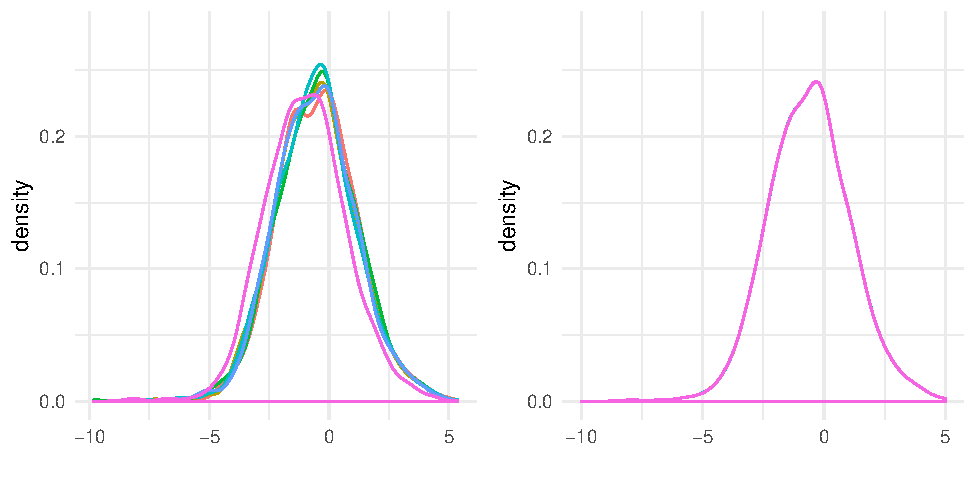
\includegraphics[width=0.8\linewidth]{bspr-workshop-2018_files/figure-latex/compare-normalisation-1} 

}

\caption{Comparison of the protein distributions before
normalization (left) and after quantile normalization (right).}\label{fig:compare-normalisation}
\end{figure}

\begin{enumerate}
\def\labelenumi{\arabic{enumi}.}
\setcounter{enumi}{2}
\tightlist
\item
  Use \texttt{t.test} to perform Welch Two Sample t-test on
  untransformed data. This outputs the p-values we need for each
  protein.
\end{enumerate}

\begin{Shaded}
\begin{Highlighting}[]
\CommentTok{# T-test function for multiple experiments}
\NormalTok{expriments_ttest <-}\StringTok{ }\ControlFlowTok{function}\NormalTok{(dt,grp1,grp2)\{}
  \CommentTok{# Subset control group and convert to numeric}
\NormalTok{  x <-}\StringTok{ }\NormalTok{dt[grp1] }\OperatorTok\StringTok{ }\NormalTok{unlist }\OperatorTok\StringTok{ }\KeywordTok{as.numeric}\NormalTok{()}
  \CommentTok{# Subset treatment group and convert to numeric}
\NormalTok{  y <-}\StringTok{ }\NormalTok{dt[grp2] }\OperatorTok\StringTok{ }\NormalTok{unlist }\OperatorTok\StringTok{ }\KeywordTok{as.numeric}\NormalTok{()}
  \CommentTok{# Perform t-test}
\NormalTok{  result <-}\StringTok{ }\KeywordTok{t.test}\NormalTok{(x, y)}
  \CommentTok{# Return p-values}
  \KeywordTok{return}\NormalTok{(result}\OperatorTok{$}\NormalTok{p.value)}
\NormalTok{\} }
\end{Highlighting}
\end{Shaded}

\begin{Shaded}
\begin{Highlighting}[]
\CommentTok{# Apply t-test function to data}
\CommentTok{# array = dat, 1 = rows, FUN = expriments_ttest, and arguements}
\CommentTok{# For median normalised data}
\NormalTok{p_vals <-}\StringTok{ }\KeywordTok{apply}\NormalTok{(dat_norm,}\DecValTok{1}\NormalTok{,expriments_ttest, }\DataTypeTok{grp1 =} \KeywordTok{c}\NormalTok{(}\DecValTok{3}\OperatorTok{:}\DecValTok{5}\NormalTok{), }\DataTypeTok{grp2 =} \KeywordTok{c}\NormalTok{(}\DecValTok{6}\OperatorTok{:}\DecValTok{8}\NormalTok{))}

\NormalTok{p_vals_max <-}\StringTok{ }\KeywordTok{apply}\NormalTok{(dat_norm_max,}\DecValTok{1}\NormalTok{,expriments_ttest, }\DataTypeTok{grp1 =} \KeywordTok{c}\NormalTok{(}\DecValTok{3}\OperatorTok{:}\DecValTok{5}\NormalTok{), }\DataTypeTok{grp2 =} \KeywordTok{c}\NormalTok{(}\DecValTok{6}\OperatorTok{:}\DecValTok{8}\NormalTok{))}

\CommentTok{# Plot histograms}
\KeywordTok{hist}\NormalTok{(p_vals)}
\end{Highlighting}
\end{Shaded}

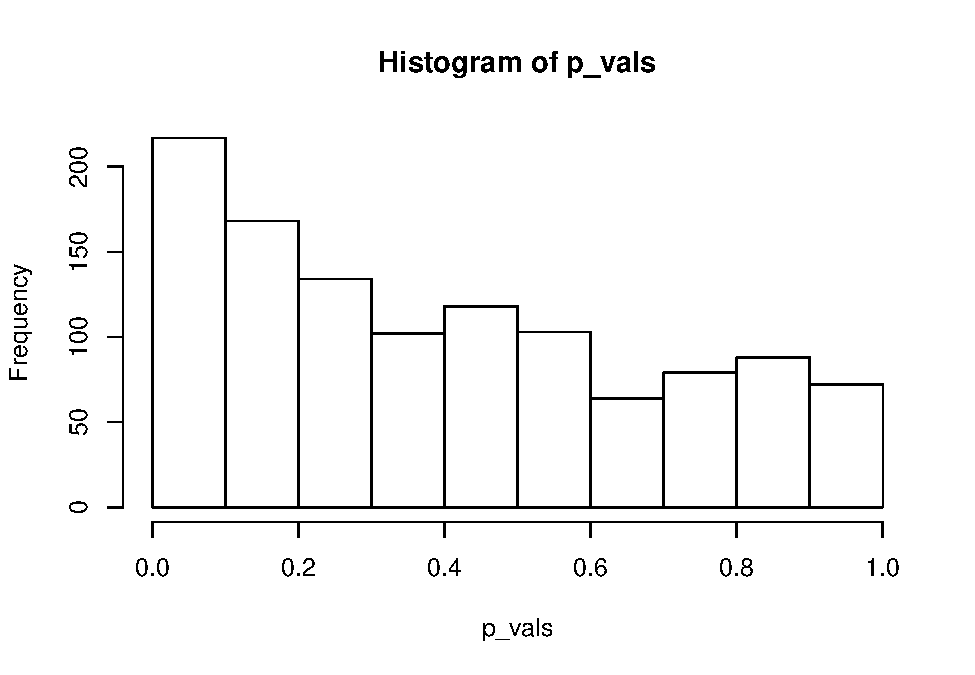
\includegraphics{bspr-workshop-2018_files/figure-latex/t-tests-1.pdf}

\begin{Shaded}
\begin{Highlighting}[]
\KeywordTok{hist}\NormalTok{(p_vals_max)}
\end{Highlighting}
\end{Shaded}

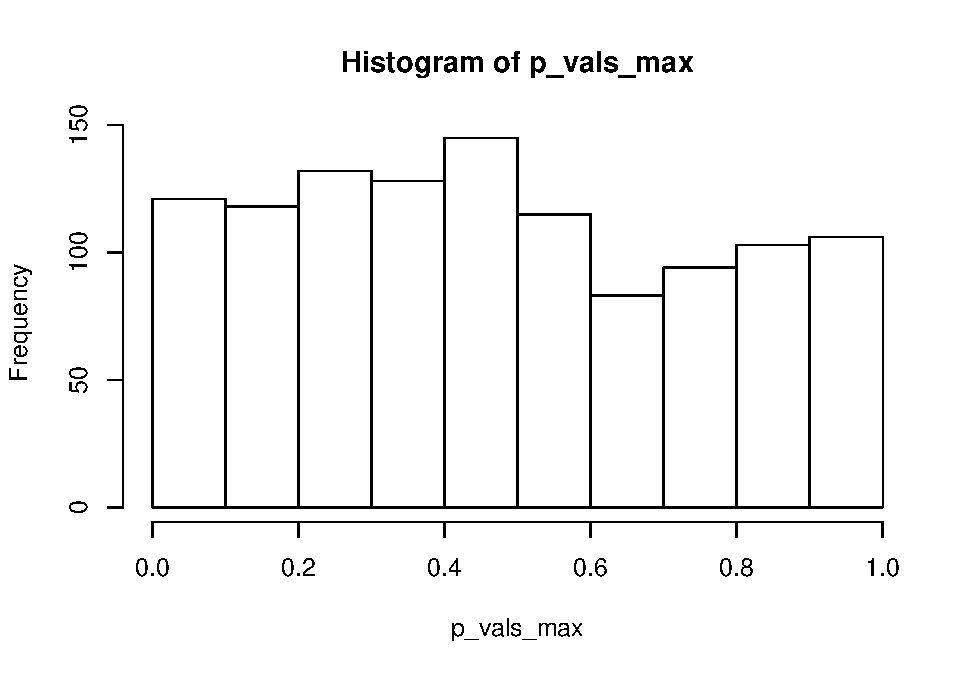
\includegraphics{bspr-workshop-2018_files/figure-latex/t-tests-2.pdf}

\begin{enumerate}
\def\labelenumi{\arabic{enumi}.}
\setcounter{enumi}{3}
\tightlist
\item
  Perform log transformation of the observations for each protein.
\end{enumerate}

\begin{Shaded}
\begin{Highlighting}[]
\CommentTok{# Select columns and log data}
\NormalTok{dat_log <-}\StringTok{ }\NormalTok{dat_norm }\OperatorTok\StringTok{ }
\StringTok{  }\KeywordTok{select}\NormalTok{(}\OperatorTok{-}\KeywordTok{c}\NormalTok{(protein_accession,protein_description)) }\OperatorTok\StringTok{ }\KeywordTok{log2}\NormalTok{()}
\NormalTok{dat_max_log <-}\StringTok{ }\NormalTok{dat_norm_max }\OperatorTok
\StringTok{  }\KeywordTok{select}\NormalTok{(}\OperatorTok{-}\KeywordTok{c}\NormalTok{(protein_accession,protein_description)) }\OperatorTok\StringTok{ }\KeywordTok{log2}\NormalTok{()}
\end{Highlighting}
\end{Shaded}

\begin{enumerate}
\def\labelenumi{\arabic{enumi}.}
\setcounter{enumi}{4}
\tightlist
\item
  Calculate the mean observation for each protein under each condition.
\end{enumerate}

\begin{Shaded}
\begin{Highlighting}[]
\NormalTok{con <-}\StringTok{ }\KeywordTok{apply}\NormalTok{(dat_log[,}\DecValTok{1}\OperatorTok{:}\DecValTok{3}\NormalTok{],}\DecValTok{1}\NormalTok{,mean)}
\NormalTok{trt <-}\StringTok{ }\KeywordTok{apply}\NormalTok{(dat_log[,}\DecValTok{4}\OperatorTok{:}\DecValTok{6}\NormalTok{],}\DecValTok{1}\NormalTok{,mean)}

\NormalTok{con_max <-}\StringTok{ }\KeywordTok{apply}\NormalTok{(dat_max_log[,}\DecValTok{1}\OperatorTok{:}\DecValTok{3}\NormalTok{],}\DecValTok{1}\NormalTok{,mean)}
\NormalTok{trt_max <-}\StringTok{ }\KeywordTok{apply}\NormalTok{(dat_max_log[,}\DecValTok{4}\OperatorTok{:}\DecValTok{6}\NormalTok{],}\DecValTok{1}\NormalTok{,mean)}
\end{Highlighting}
\end{Shaded}

\begin{enumerate}
\def\labelenumi{\arabic{enumi}.}
\setcounter{enumi}{5}
\tightlist
\item
  The log fold change is then the difference between condition 1 and
  condition 2.
\end{enumerate}

\begin{Shaded}
\begin{Highlighting}[]
\CommentTok{# Plot a histogram to look at the distribution.}

\CommentTok{# Calculate fold change}
\NormalTok{dat_fc <-}\StringTok{ }\NormalTok{con }\OperatorTok{-}\StringTok{ }\NormalTok{trt}
\NormalTok{dat_max_fc <-}\StringTok{ }\NormalTok{con_max }\OperatorTok{-}\StringTok{ }\NormalTok{trt_max}

\CommentTok{# Plot histograms}
\KeywordTok{hist}\NormalTok{(dat_fc)}
\end{Highlighting}
\end{Shaded}

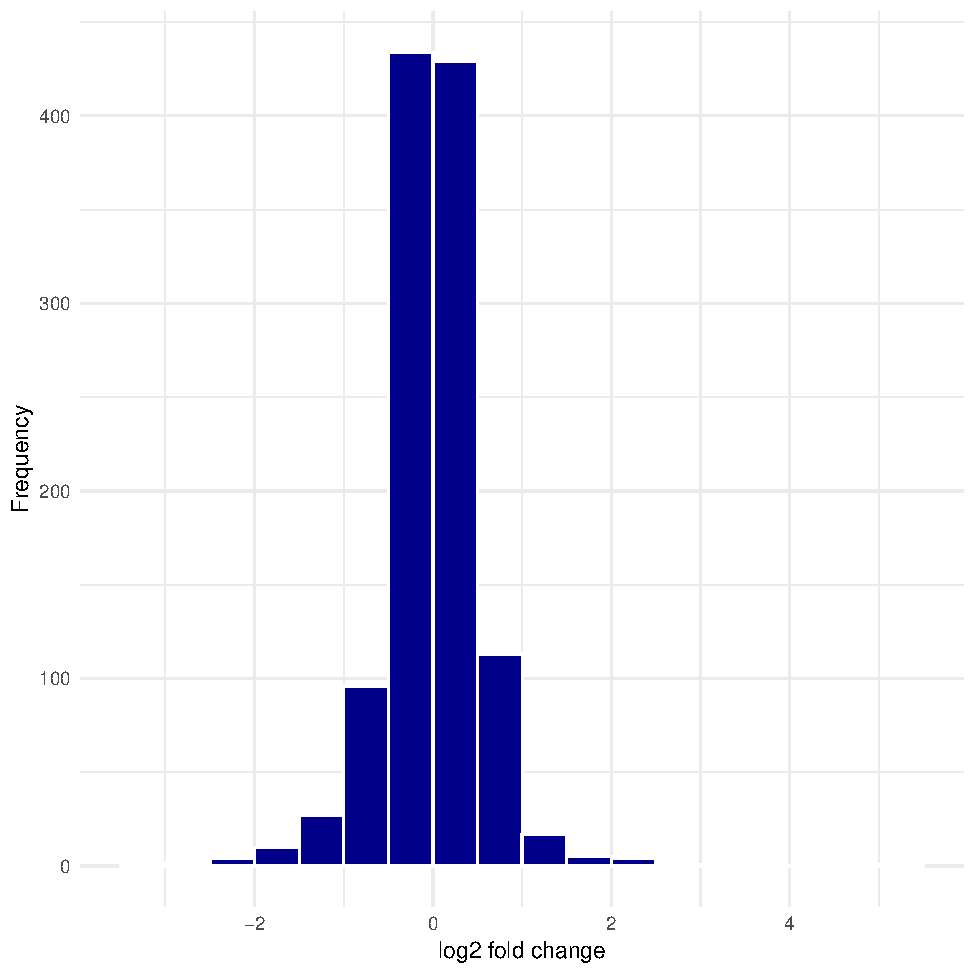
\includegraphics{bspr-workshop-2018_files/figure-latex/log-fc-1.pdf}

\begin{Shaded}
\begin{Highlighting}[]
\KeywordTok{hist}\NormalTok{(dat_max_fc)}
\end{Highlighting}
\end{Shaded}

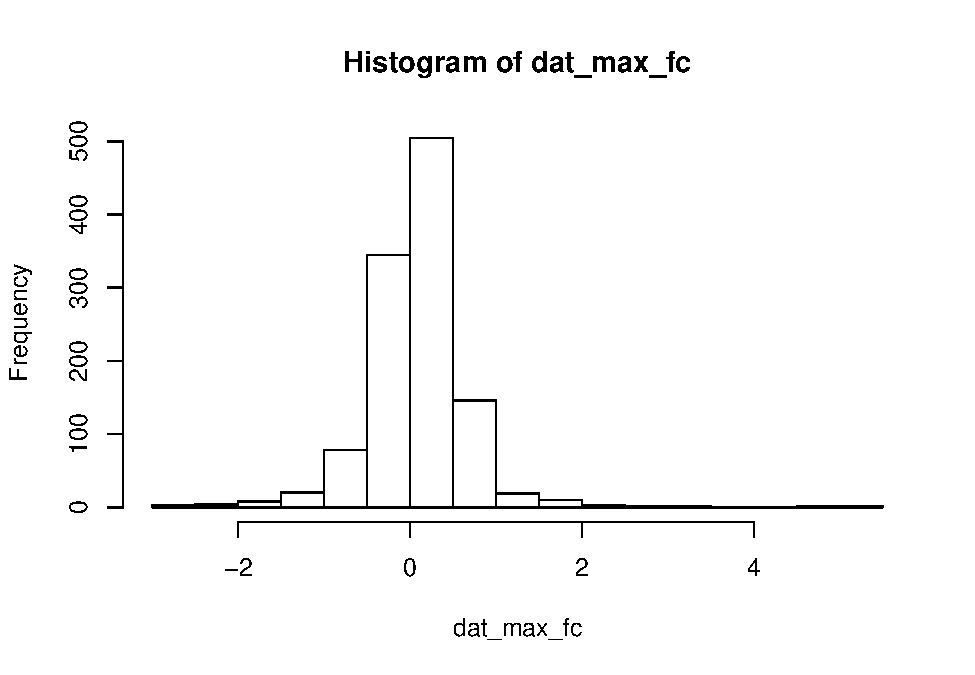
\includegraphics{bspr-workshop-2018_files/figure-latex/log-fc-2.pdf}

\section{Visualising data}\label{visualising-data}

Based on empircal research, there are some general rules on
visulisations that are worth bearing in mind:

\begin{enumerate}
\def\labelenumi{\arabic{enumi}.}
\tightlist
\item
  Plot
\end{enumerate}

\section{Creating a volcano plot}\label{creating-a-volcano-plot}

A volcano plot is a plot of the log fold change in the observation
between two conditions on the x-axis, for example the protein expression
between treatment and control conditions. On the y-axis is the
corresponding p-value for each observation, representing the likelihood
that an observed change is due to the different conditions rather than
arising from a natural variation in the fold change that might be
observed if we performed many replications of the experiment.

The aim of a volcano plot is to enable the viewer to quickly see the
effect (if any) of an experiment with two conditions on many species
(i.e.~proteins) in terms of both an increase and decrease of the
observed value.

Like all plots it has it's good and bad points, namely it's good that we
can visualise a lot of complex information in one plot. However this is
also it's main weakness, it's rather complicated to understand in one
glance.

However, volcano plots are widely used in the literature, so there may
be an amount of \href{https://en.wikipedia.org/wiki/Social_proof}{social
proof} giving rise to their popularity as opposed to their utility.

\begin{Shaded}
\begin{Highlighting}[]
\NormalTok{dat_vplot <-}\StringTok{ }\KeywordTok{tibble}\NormalTok{(}\DataTypeTok{prots=}\NormalTok{ dat_norm}\OperatorTok{$}\NormalTok{protein_accession,}
                   \DataTypeTok{logfc =}\NormalTok{ dat_fc,}
                   \DataTypeTok{pval =} \OperatorTok{-}\DecValTok{1}\OperatorTok{*}\KeywordTok{log10}\NormalTok{(p_vals))}

\NormalTok{dat_max <-}\StringTok{ }\KeywordTok{tibble}\NormalTok{(}\DataTypeTok{prots=}\NormalTok{ dat_norm_max}\OperatorTok{$}\NormalTok{protein_accession,}
                      \DataTypeTok{logfc =}\NormalTok{ dat_max_fc,}
                      \DataTypeTok{pval =} \OperatorTok{-}\DecValTok{1}\OperatorTok{*}\KeywordTok{log10}\NormalTok{(p_vals_max))}

\NormalTok{dat_max }\OperatorTok\StringTok{ }\KeywordTok{ggplot}\NormalTok{(}\KeywordTok{aes}\NormalTok{(logfc,pval)) }\OperatorTok{+}\StringTok{ }\KeywordTok{geom_point}\NormalTok{()}
\end{Highlighting}
\end{Shaded}

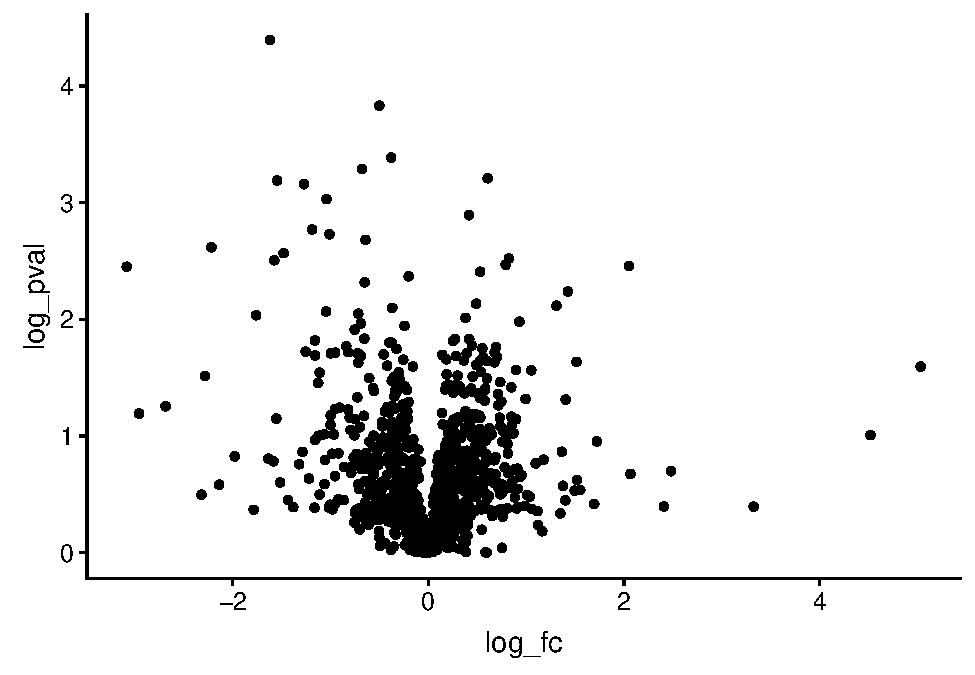
\includegraphics{bspr-workshop-2018_files/figure-latex/volcano-plot-1.pdf}

\begin{Shaded}
\begin{Highlighting}[]
\NormalTok{dat_vplot }\OperatorTok
\StringTok{  }\CommentTok{# Add a threhold for significant observations}
\StringTok{  }\KeywordTok{mutate}\NormalTok{(}\DataTypeTok{threshold =} \KeywordTok{if_else}\NormalTok{(logfc }\OperatorTok{>=}\StringTok{ }\DecValTok{2} \OperatorTok{&}\StringTok{ }\NormalTok{pval }\OperatorTok{>=}\StringTok{ }\FloatTok{1.5} \OperatorTok{|}
\StringTok{                               }\NormalTok{logfc }\OperatorTok{<=}\StringTok{ }\OperatorTok{-}\DecValTok{2} \OperatorTok{&}\StringTok{ }\NormalTok{pval }\OperatorTok{>=}\StringTok{ }\FloatTok{1.5}\NormalTok{,}\StringTok{"A"}\NormalTok{, }\StringTok{"B"}\NormalTok{)) }\OperatorTok
\StringTok{  }\CommentTok{# Plot with points coloured according to the threshold}
\StringTok{  }\KeywordTok{ggplot}\NormalTok{(}\KeywordTok{aes}\NormalTok{(logfc,pval, }\DataTypeTok{colour =}\NormalTok{ threshold)) }\OperatorTok{+}
\StringTok{  }\KeywordTok{geom_point}\NormalTok{(}\DataTypeTok{alpha =} \FloatTok{0.5}\NormalTok{) }\OperatorTok{+}\StringTok{ }\CommentTok{# Alpha sets the transparency of the points}
\StringTok{  }\CommentTok{# Add dotted lines to indicate the threshold, semi-transparent}
\StringTok{  }\KeywordTok{geom_hline}\NormalTok{(}\DataTypeTok{yintercept =} \FloatTok{1.5}\NormalTok{, }\DataTypeTok{linetype =} \DecValTok{2}\NormalTok{, }\DataTypeTok{alpha =} \FloatTok{0.5}\NormalTok{) }\OperatorTok{+}\StringTok{ }
\StringTok{  }\KeywordTok{geom_vline}\NormalTok{(}\DataTypeTok{xintercept =} \DecValTok{2}\NormalTok{, }\DataTypeTok{linetype =} \DecValTok{2}\NormalTok{, }\DataTypeTok{alpha =} \FloatTok{0.5}\NormalTok{) }\OperatorTok{+}
\StringTok{  }\KeywordTok{geom_vline}\NormalTok{(}\DataTypeTok{xintercept =} \OperatorTok{-}\DecValTok{2}\NormalTok{, }\DataTypeTok{linetype =} \DecValTok{2}\NormalTok{, }\DataTypeTok{alpha =} \FloatTok{0.5}\NormalTok{) }\OperatorTok{+}
\StringTok{  }\CommentTok{# Set the colour of the points}
\StringTok{  }\KeywordTok{scale_colour_manual}\NormalTok{(}\DataTypeTok{values =} \KeywordTok{c}\NormalTok{(}\StringTok{"A"}\NormalTok{=}\StringTok{ "red"}\NormalTok{, }\StringTok{"B"}\NormalTok{=}\StringTok{ "black"}\NormalTok{)) }\OperatorTok{+}
\StringTok{  }\KeywordTok{xlab}\NormalTok{(}\StringTok{"log2 fold change"}\NormalTok{) }\OperatorTok{+}\StringTok{ }\KeywordTok{ylab}\NormalTok{(}\StringTok{"-log10 p-value"}\NormalTok{) }\OperatorTok{+}\StringTok{ }\CommentTok{# Relabel the axes}
\StringTok{  }\KeywordTok{theme_minimal}\NormalTok{() }\OperatorTok{+}\StringTok{ }\CommentTok{# Set the theme}
\StringTok{  }\KeywordTok{theme}\NormalTok{(}\DataTypeTok{legend.position=}\StringTok{"none"}\NormalTok{) }\CommentTok{# Hide the legend}
\end{Highlighting}
\end{Shaded}

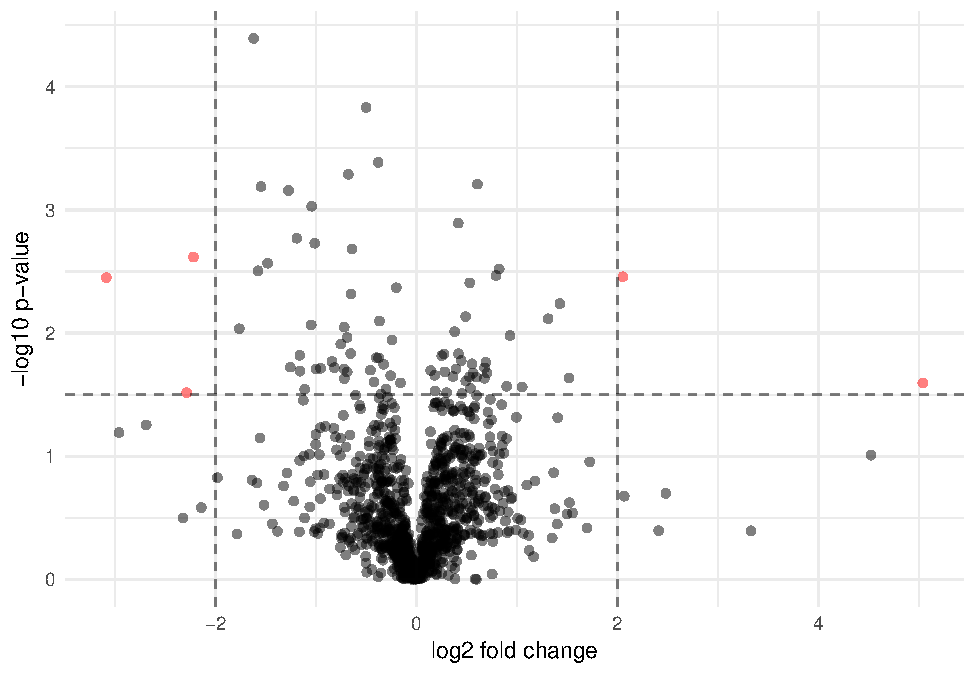
\includegraphics{bspr-workshop-2018_files/figure-latex/volcano-plot-2.pdf}

But which proteins are the significant observations?

\begin{Shaded}
\begin{Highlighting}[]
\NormalTok{dat_vplot }\OperatorTok
\StringTok{  }\CommentTok{# Add a threhold for significant observations}
\StringTok{  }\KeywordTok{mutate}\NormalTok{(}\DataTypeTok{threshold =} \KeywordTok{if_else}\NormalTok{(logfc }\OperatorTok{>=}\StringTok{ }\DecValTok{2} \OperatorTok{&}\StringTok{ }\NormalTok{pval }\OperatorTok{>=}\StringTok{ }\FloatTok{1.5} \OperatorTok{|}
\StringTok{                               }\NormalTok{logfc }\OperatorTok{<=}\StringTok{ }\OperatorTok{-}\DecValTok{2} \OperatorTok{&}\StringTok{ }\NormalTok{pval }\OperatorTok{>=}\StringTok{ }\FloatTok{1.5}\NormalTok{,}\StringTok{"A"}\NormalTok{, }\StringTok{"B"}\NormalTok{),}
         \DataTypeTok{prot_id =} \KeywordTok{str_extract}\NormalTok{(prots,}\StringTok{".\{6\}$"}\NormalTok{)) }\OperatorTok\StringTok{  }\CommentTok{# Get last six characters}
\StringTok{  }\CommentTok{# Filter observations above the threshold}
\StringTok{  }\KeywordTok{filter}\NormalTok{(threshold }\OperatorTok{==}\StringTok{ "A"}\NormalTok{)}
\end{Highlighting}
\end{Shaded}

\begin{verbatim}
## # A tibble: 5 x 5
##   prots               logfc  pval threshold prot_id
##   <chr>               <dbl> <dbl> <chr>     <chr>  
## 1 AKA12_HUMAN_Q02952  -2.29  1.52 A         Q02952 
## 2 GFPT2_HUMAN_O94808  -3.09  2.45 A         O94808 
## 3 H7BYV1_HUMAN_H7BYV1  2.05  2.46 A         H7BYV1 
## 4 ITAV_HUMAN_P06756   -2.22  2.62 A         P06756 
## 5 CHD5_HUMAN_Q8TDI0    5.04  1.60 A         Q8TDI0
\end{verbatim}

\section{Creating a heatmap plot}\label{creating-a-heatmap-plot}

\begin{Shaded}
\begin{Highlighting}[]
\NormalTok{dat_mut <-}\StringTok{ }\NormalTok{dat_norm }\OperatorTok
\StringTok{  }\KeywordTok{mutate}\NormalTok{(}\DataTypeTok{pval =}\NormalTok{ dat_vplot}\OperatorTok{$}\NormalTok{pval, }\DataTypeTok{logfc =}\NormalTok{ dat_vplot}\OperatorTok{$}\NormalTok{logfc) }\OperatorTok
\StringTok{  }\KeywordTok{filter}\NormalTok{(pval }\OperatorTok{>=}\StringTok{ }\DecValTok{2} \OperatorTok{&}\StringTok{ }\NormalTok{(logfc }\OperatorTok{>=}\DecValTok{2} \OperatorTok{|}\StringTok{ }\NormalTok{logfc }\OperatorTok{<=}\StringTok{ }\DecValTok{2}\NormalTok{)) }\OperatorTok
\StringTok{  }\KeywordTok{select}\NormalTok{(}\OperatorTok{-}\KeywordTok{c}\NormalTok{(}\DecValTok{2}\NormalTok{,}\DecValTok{9}\OperatorTok{:}\DecValTok{10}\NormalTok{))}

\NormalTok{dat_sel <-}\StringTok{ }\KeywordTok{as.matrix.data.frame}\NormalTok{(dat_mut[,}\DecValTok{2}\OperatorTok{:}\DecValTok{7}\NormalTok{]) }\OperatorTok\StringTok{ }\KeywordTok{log2}\NormalTok{()}
\KeywordTok{row.names}\NormalTok{(dat_sel) <-}\StringTok{ }\NormalTok{dat_mut}\OperatorTok{$}\NormalTok{protein_accession}

\NormalTok{dat.tn <-}\StringTok{ }\KeywordTok{scale}\NormalTok{(}\KeywordTok{t}\NormalTok{(dat_sel)) }\OperatorTok\StringTok{ }\KeywordTok{t}\NormalTok{()}
\CommentTok{#dat.tn <- t(dat.n)}
\CommentTok{#dat.tn <- dat_sel}

\CommentTok{#gplots::heatmap.2(dat.tn, scale = 'row',trace="none")}
\KeywordTok{library}\NormalTok{(pheatmap)}
\KeywordTok{pheatmap}\NormalTok{(dat.tn,}\DataTypeTok{cutree_rows =} \DecValTok{2}\NormalTok{,}
         \DataTypeTok{cutree_cols =} \DecValTok{2}\NormalTok{)}
\end{Highlighting}
\end{Shaded}

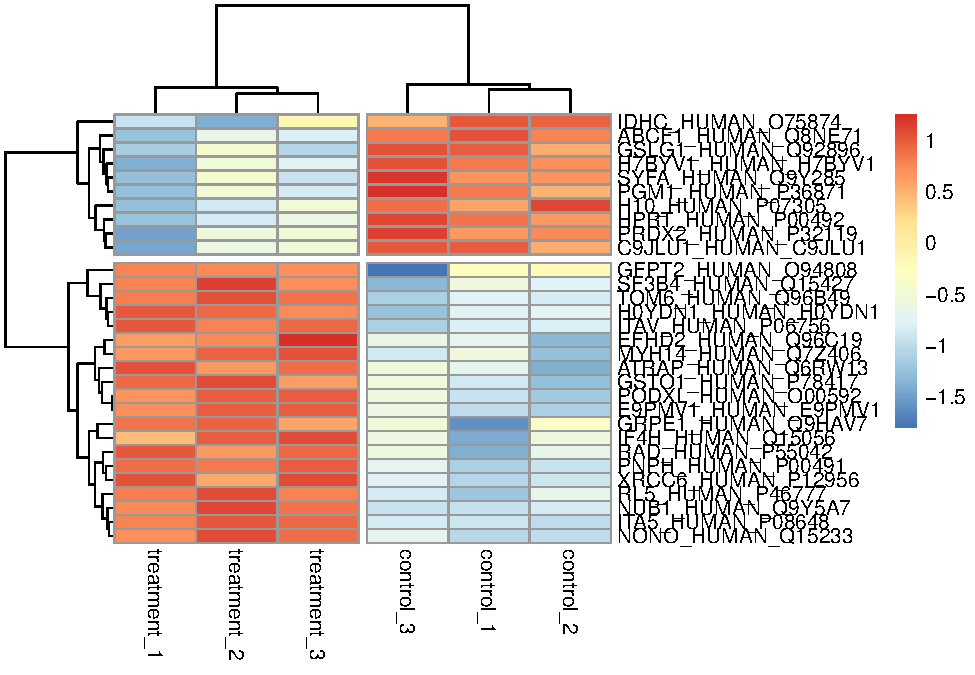
\includegraphics{bspr-workshop-2018_files/figure-latex/heatmap-2-1.pdf}

\begin{Shaded}
\begin{Highlighting}[]
\NormalTok{cal_z_score <-}\StringTok{ }\ControlFlowTok{function}\NormalTok{(x)\{}
\NormalTok{  (x }\OperatorTok{-}\StringTok{ }\KeywordTok{mean}\NormalTok{(x)) }\OperatorTok{/}\StringTok{ }\KeywordTok{sd}\NormalTok{(x)}
\NormalTok{\}}

\NormalTok{data_subset_norm <-}\StringTok{ }\KeywordTok{t}\NormalTok{(}\KeywordTok{apply}\NormalTok{(dat_mut[,}\DecValTok{2}\OperatorTok{:}\DecValTok{7}\NormalTok{], }\DecValTok{1}\NormalTok{, cal_z_score))}
\KeywordTok{row.names}\NormalTok{(data_subset_norm) <-}\StringTok{ }\NormalTok{dat_mut}\OperatorTok{$}\NormalTok{protein_accession}
\KeywordTok{pheatmap}\NormalTok{(data_subset_norm)}
\end{Highlighting}
\end{Shaded}

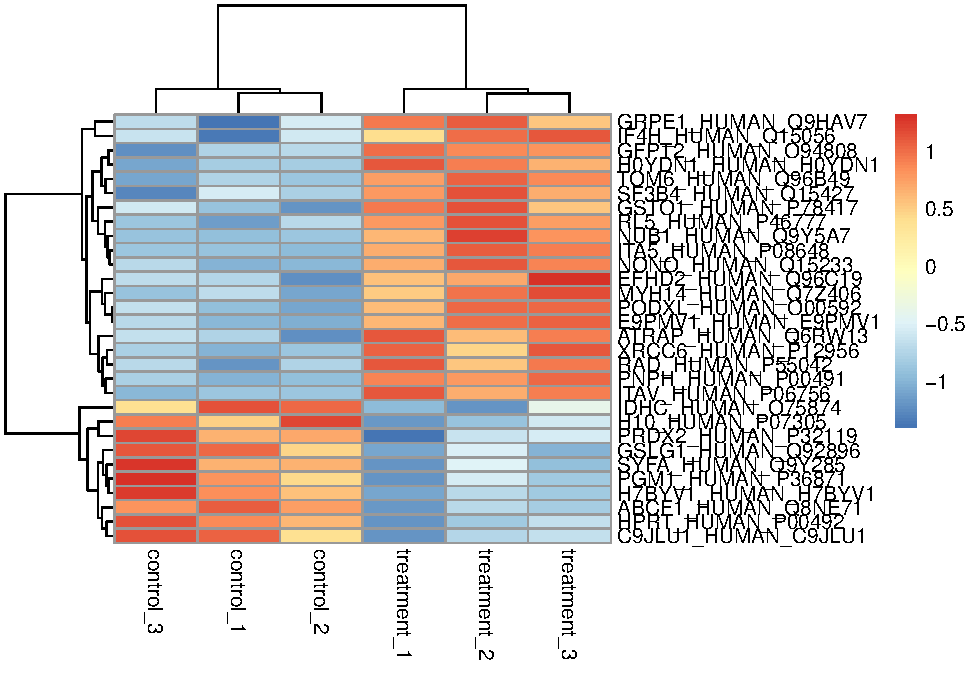
\includegraphics{bspr-workshop-2018_files/figure-latex/heatmap-2-2.pdf}

\begin{Shaded}
\begin{Highlighting}[]
\NormalTok{d1 <-}\StringTok{ }\NormalTok{dat.tn }\OperatorTok\StringTok{ }\KeywordTok{t}\NormalTok{() }\OperatorTok
\StringTok{  }\KeywordTok{dist}\NormalTok{(.,}\DataTypeTok{method =} \StringTok{"euclidean"}\NormalTok{, }\DataTypeTok{diag =} \OtherTok{FALSE}\NormalTok{, }\DataTypeTok{upper =} \OtherTok{FALSE}\NormalTok{)}

\NormalTok{d2 <-}\StringTok{ }\NormalTok{dat.tn }\OperatorTok
\StringTok{  }\KeywordTok{dist}\NormalTok{(.,}\DataTypeTok{method =} \StringTok{"euclidean"}\NormalTok{, }\DataTypeTok{diag =} \OtherTok{FALSE}\NormalTok{, }\DataTypeTok{upper =} \OtherTok{FALSE}\NormalTok{)}

\CommentTok{# Clustering distance between experiments using Ward linkage}
\NormalTok{c1 <-}\StringTok{ }\KeywordTok{hclust}\NormalTok{(d1, }\DataTypeTok{method =} \StringTok{"ward.D2"}\NormalTok{, }\DataTypeTok{members =} \OtherTok{NULL}\NormalTok{)}
\CommentTok{# Clustering distance between proteins using Ward linkage}
\NormalTok{c2 <-}\StringTok{ }\KeywordTok{hclust}\NormalTok{(d2, }\DataTypeTok{method =} \StringTok{"ward.D2"}\NormalTok{, }\DataTypeTok{members =} \OtherTok{NULL}\NormalTok{)}

\CommentTok{# Check clustering by plotting dendrograms}
\KeywordTok{par}\NormalTok{(}\DataTypeTok{mfrow=}\KeywordTok{c}\NormalTok{(}\DecValTok{2}\NormalTok{,}\DecValTok{1}\NormalTok{),}\DataTypeTok{cex=}\FloatTok{0.5}\NormalTok{) }\CommentTok{# Make 2 rows, 1 col plot frame and shrink labels}
\KeywordTok{plot}\NormalTok{(c1); }\KeywordTok{plot}\NormalTok{(c2) }\CommentTok{# Plot both cluster dendrograms}
\end{Highlighting}
\end{Shaded}

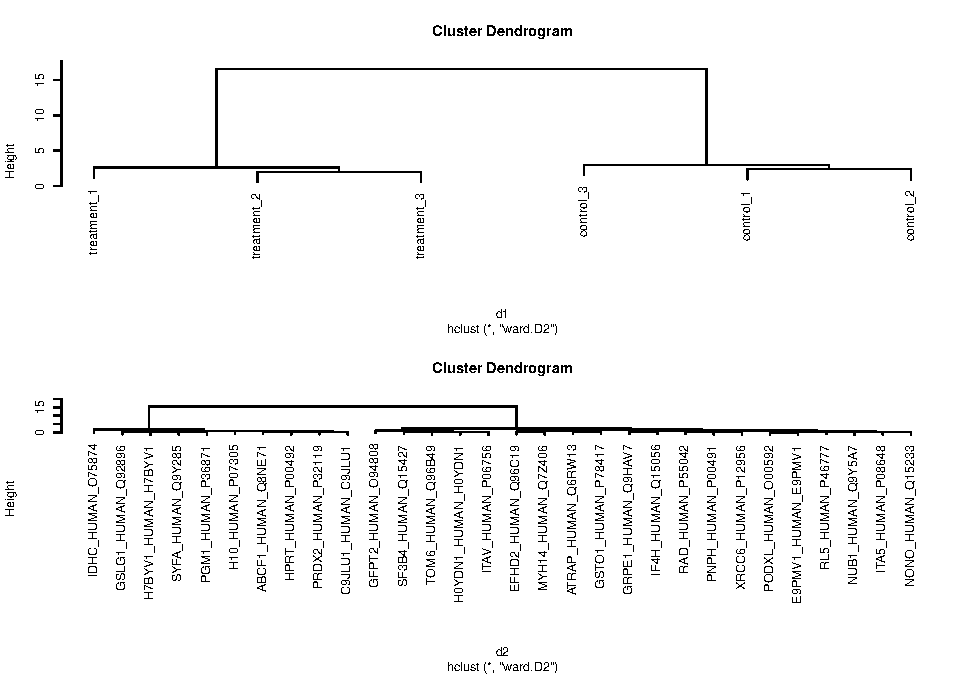
\includegraphics{bspr-workshop-2018_files/figure-latex/heatmap-2-3.pdf}

\begin{Shaded}
\begin{Highlighting}[]
\CommentTok{# Set colours for heatmap, 25 increments}
\NormalTok{my_palette <-}\StringTok{ }\KeywordTok{colorRampPalette}\NormalTok{(}\KeywordTok{c}\NormalTok{(}\StringTok{"blue"}\NormalTok{,}\StringTok{"white"}\NormalTok{,}\StringTok{"red"}\NormalTok{))(}\DataTypeTok{n =} \DecValTok{25}\NormalTok{)}

\CommentTok{# Plot heatmap with heatmap.2}
\KeywordTok{par}\NormalTok{(}\DataTypeTok{cex.main=}\FloatTok{0.75}\NormalTok{) }\CommentTok{# Shrink title fonts on plot}
\NormalTok{gplots}\OperatorTok{::}\KeywordTok{heatmap.2}\NormalTok{(dat.tn,                     }\CommentTok{# Tidy, normalised data}
          \DataTypeTok{Colv=}\KeywordTok{as.dendrogram}\NormalTok{(c1),     }\CommentTok{# Experiments clusters in cols}
          \DataTypeTok{Rowv=}\KeywordTok{as.dendrogram}\NormalTok{(c2),     }\CommentTok{# Protein clusters in rows}
          \DataTypeTok{density.info=}\StringTok{"histogram"}\NormalTok{,   }\CommentTok{# Plot histogram of data and colour key}
          \DataTypeTok{trace=}\StringTok{"none"}\NormalTok{,               }\CommentTok{# Turn of trace lines from heat map}
          \DataTypeTok{col =}\NormalTok{ my_palette,           }\CommentTok{# Use my colour scheme}
          \DataTypeTok{cexRow=}\FloatTok{0.5}\NormalTok{,}\DataTypeTok{cexCol=}\FloatTok{0.75}\NormalTok{)     }\CommentTok{# Amend row and column label fonts}
\end{Highlighting}
\end{Shaded}

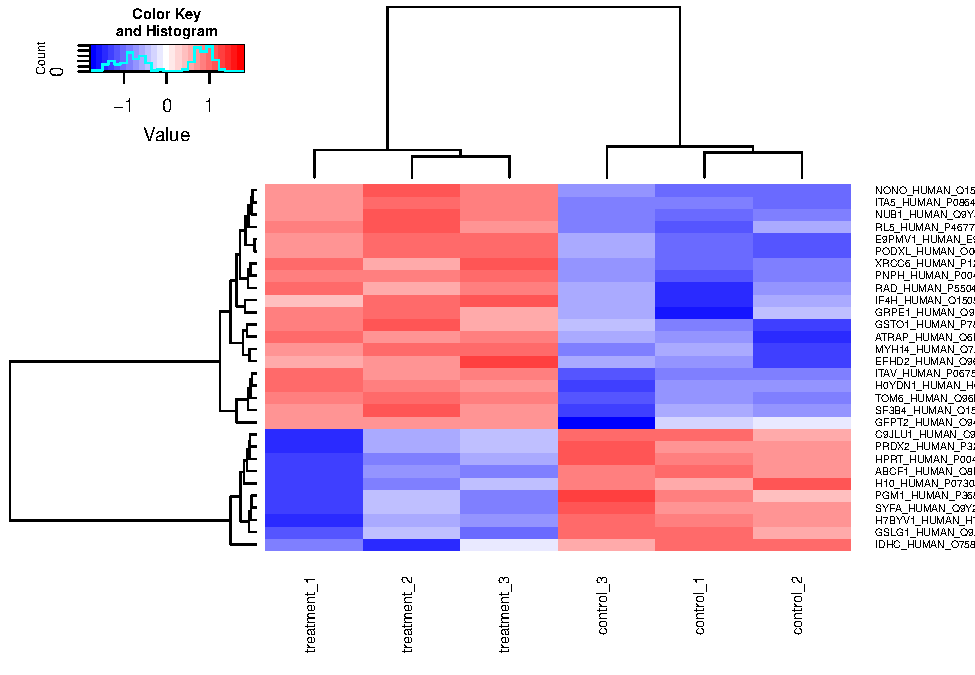
\includegraphics{bspr-workshop-2018_files/figure-latex/heatmap-1-1.pdf}

\chapter{Going further}\label{going-further}

\section{\texorpdfstring{Learning \texttt{dplyr}
verbs}{Learning dplyr verbs}}\label{learning-dplyr-verbs}

\section{Getting help and joining the R
community}\label{getting-help-and-joining-the-r-community}

\section{Communication: creating reports, presentations and
websites}\label{communication-creating-reports-presentations-and-websites}

\bibliography{packages.bib,book.bib}


\end{document}
